\chapter{Model Development}
\label{ch:ModelDev}

\section{Bond Pair Material Model}
Consider the material model illustrated in \cref{fig:SimpleBondpair} in which every bond-vector originating from a point is connected by a rotational spring to its opposite originating from that same point.
%
\begin{figure}[h]
\centering
\resizebox{0.6\linewidth}{!}{\subinputfrom{\diagrampath}{simpleBondPair.eps_tex}}
\caption{Illustration of a bond pair model that resists angular deformation}
\label{fig:SimpleBondpair}
\end{figure}
%
If we call the deformed angle between these bonds \(\theta\), and choose the potential energy of that spring to be \(w(\boldsymbol{\xi}) = \omega(\boldsymbol{\xi})\alpha [1 + \cos(\theta) ] \) for the bond pair $\boldsymbol{\xi}$ and $-\boldsymbol{\xi}$, we can recover the non-ordinary force state proposed by Silling in \cite{silling2007peridynamic} by taking the Fr\'echet derivative. For the derivation and a description of the Fr\'echet derivative see \cref{sec:frechet}.
%
\begin{align}
\label{eq:SillingForceNO}
\vstate{T}{}{\boldsymbol{\xi}} &= \nabla w\!\left(\vstate{Y}{}{\boldsymbol{\xi}}\right)\notag \\
%
&=\omega(\boldsymbol{\xi})\frac{-\alpha}{|\vstate{Y}{}{\boldsymbol{\xi}}|} \frac{\vstate{Y}{}{\boldsymbol{\xi}}}{|\vstate{Y}{}{\boldsymbol{\xi}}|} \times \left[\frac{\vstate{Y}{}{\boldsymbol{\xi}}}{|\vstate{Y}{}{\boldsymbol{\xi}}|} \times \frac{\vstate{Y}{}{-\boldsymbol{\xi}}}{|\vstate{Y}{}{-\boldsymbol{\xi}}|}\right]
\end{align}
%
Though it looks complex, \cref{eq:SillingForceNO} indicates a bond force perpendicular to the deformed bond and in the plane containing both the deformed bond and its partner as illustrated in \cref{fig:Bondpair}. 
The force magnitude is proportional to the sine of the angle between the bonds divided by the length of the deformed bond. 
%
\begin{figure}[h]
\centering
\resizebox{0.6\linewidth}{!}{\subinputfrom{\diagrampath}{bondPair.eps_tex}}
\caption{Deformation and force vector states}
\label{fig:Bondpair}
\end{figure}
%
This response is consistent with the idea of a rotational spring between bonds as long as the change in angle is small. 
Because the potential energy and force states are functions of \textit{pairs} of peridynamic bonds, we will call this formulation a \textit{bond-pair model}. 
Other choices for the bond-pair potential function, such as $w = (\pi - \theta)^2$, are also possible, but result in more mathematically complex analysis.

\section{Bond Pair Beam in Bending}
\label{sec:BPbeam}
The simplest application of our bond-pair based peridynamic model is that of \cref{fig:continuousbeam}, a beam in transverse bending.
Much of the material in this section can also be found in \cite{ogrady2014beams}.
%
\begin{figure}[h]
  \centering
\subinputfrom{\diagrampath}{continuousBeam.eps_tex}
\caption{A continuous peridynamic beam with horizon $\delta$}
\label{fig:continuousbeam}
\end{figure}
%

\subsection{Energy Equivalence}
\label{sec:beamEnergy}
To determine an appropriate choice of $\alpha$ for \cref{eq:SillingForceNO}, we desire our peridynamic model to have an equivalent strain energy density to a classical Euler-Bernoulli beam in the \emph{local limit}, i.e.\ when the nonlocal length scale vanishes.  We will begin with the assumptions from Euler beam theory: the length of the beam is much greater than thickness, vertical displacements are small, and rotations are small. For small vertical displacements (i.e.\ $\sin{\theta} \approx \theta$) we have
%
\begin{equation}
\theta(\vstate{Y}{}{\xi},\vstate{Y}{}{\mathbf{-\xi}}) \approx \pi-\frac{v(x+\xi)-2v(x)+v(x-\xi)}{\xi},
\label{eq:beamdtheta}
\end{equation}
%
where $v$ is the vertical displacement of material point.  Momentarily assuming that $v$ is continuous and using a Taylor series to expand the right-hand-side of eq.~(\ref{eq:beamdtheta})  
%
\begin{align}
\theta(\vstate{Y}{}{\xi},\vstate{Y}{}{\mathbf{-\xi}}) &\approx \pi-\xi \frac{\partial^2 v}{\partial x^2}+\mathcal{O}(\xi^3) \notag \\
&\approx  \pi-\xi \kappa +\mathcal{O}(\xi^3); 
\label{eq:beamdtheta2}
\end{align}
with
\begin{equation}
\kappa = \frac{\partial^2 v}{\partial x^2}.\notag
\end{equation}
%
Substituting eq.~(\ref{eq:beamdtheta2}) into the equation for the strain energy density of a single bond-pair,
%
\begin{align}
\label{eq:continuousBeamw}
w(\xi) &= \omega(\xi) \alpha \left[1+\cos(\theta(\vstate{Y}{}{\xi},\vstate{Y}{}{\mathbf{-\xi}})) \right] \notag\\
&\approx \omega(\xi) \alpha\frac{\xi^2}{2}(\kappa)^2 +\mathcal{O}(\xi^4).\notag
\end{align}
%
If we use a weighting function \(\omega(\xi)=\omega(|\xi|)\) and assume that the $\omega$ plays the role of a localization kernel, i.e. $\omega = 0 \,\, \forall \,\, \xi > \delta$, the resulting strain energy density, $W$, for any material point in the peridynamic beam is
%
\begin{equation}
W = \frac{\alpha}{2}\kappa^2 \int_{-\delta}^\delta \omega(\xi)\xi^2 {\rm d}\xi + \mathcal{O}(\delta^5).\notag
\end{equation}
%
Equating $W$ with the classical Euler-Bernoulli beam strain-energy density, $\Omega$, and taking the limit as $\delta \to 0$ we can solve for $\alpha$
%
\begin{align}
    \lim_{\delta \to 0}  W &= \Omega, \notag \\
    \frac{\alpha}{2} m \kappa^2 &= \frac{EI}{2} \kappa^2, \notag \\
    \alpha &= \frac{EI}{m},
\label{eq:alpha}
\end{align}
%
with 
\begin{equation}
    m = \int_{-\delta}^{\delta} \omega(\xi) \xi^2 {\rm d}\xi \notag.
\end{equation}

While this demonstrates the model's equivalence to a linearly-elastic Euler beam, if we keep an additional term from the Taylor series approximation of \cref{eq:beamdtheta}, we recover a slightly more complex expressions for change in angle that is demonstrated in \ref{sec:EringenCompare} to reproduce an Euler beam governed by Eringen's model of nonlocal elasticity.

\subsection{Relation to Eringen Nonlocality}
\label{sec:EringenCompare}
%If we relax our homogeneity assumption somewhat, we recover from \cref{eq:beamdtheta} slightly more complex expressions for change in angle
If we keep an additional term from the Taylor series approximation of \cref{eq:beamdtheta}, we recover a slightly more complex expressions for change in angle
%
\begin{equation}
\label{eq:beamdthetaHOT}
%\theta(\vstate{Y}{}{\xi},\vstate{Y}{}{\mathbf{-\xi}}) \approx \pi-\xi \frac{\partial^2 y}{\partial x^2} -\frac{\xi^3}{12} \frac{\partial^4 y}{\partial x^4}  +\mathcal{O}(\xi^5)=  \pi-\xi \kappa-\frac{\xi^3}{12} \kappa''+\mathcal{O}(\xi^5)\notag
\theta(\vstate{Y}{}{\xi},\vstate{Y}{}{\mathbf{-\xi}}) \approx \arctan\left(\pi-\xi \frac{\partial^2 v}{\partial x^2} -\frac{\xi^3}{12} \frac{\partial^4 v}{\partial x^4}  +\mathcal{O}(\xi^5)\right)\notag
\end{equation}
%
and for the strain energy (again substituting \(\kappa = v''\) for readability),
%
%\begin{equation}
%W \approx \int_{-\delta}^\delta \omega(\xi)\alpha(\frac{\xi^2}{2}\kappa^2+\frac{\xi^4}{12}\kappa\kappa''-\frac{3\; \xi^4}{8}\kappa^4+\mathcal{O}(\xi^6)) d\xi .
%\end{equation}
%
%
\begin{equation}
%W \approx \int_{-\delta}^\delta \omega(\xi)\alpha(\frac{\xi^2}{2}\kappa^2+\frac{\xi^4}{12}\kappa\kappa''-\frac{\xi^4}{24}\kappa^4+\mathcal{O}(\xi^6)) d\xi .\notag
W \approx \int_{-\delta}^\delta \omega(\xi)\alpha(\frac{\xi^2}{2}\kappa^2+\frac{\xi^4}{12}\kappa\kappa''-\frac{3\; \xi^4}{8}\kappa^4+\mathcal{O}(\xi^6)) d\xi.\notag
\end{equation}
%
As the horizon \(\delta\) becomes small, higher-order \(\xi\) terms become relatively less important, and \(\xi^4\kappa^4\) is dominated by \(\xi^2\kappa^2\) for large \(\kappa\) and by \(\xi^4\kappa\kappa''\) for small \(\kappa\).
The remaining terms can be rearranged,
\begin{align}
W &\approx \int_{-\delta}^\delta \omega(\xi)\alpha \frac{\xi^2}{2}\kappa(\kappa + \frac{\xi^2}{6}\kappa'') d\xi, \notag
\end{align}
in a manner strongly suggesting an alternative bending resistance term.
We can picture a bending resistance based on the bond length and proportional to the nonlocal curvature  \(\bar{\kappa}=(\kappa + \frac{\xi^2}{6}\kappa'')\), so that 
%
\begin{align}
\label{eq:NLbending}
\bar{\kappa}&=(\kappa + \frac{\xi^2}{6}\kappa'') \implies  \\
W &\approx \int_{-\delta}^\delta \omega(\xi)\alpha \frac{\xi^2}{2}\kappa\bar{\kappa}d\xi .\notag
\end{align}
%  
The same analysis can be taken further to obtain higher-order energy terms with even powers of \(\xi\) and even order derivatives of \(\kappa\). 
Not all of these higher-order terms can be separated into the product of a local curvature and nonlocal bending resistance.

Eringen's model for nonlocal elasticity in \cite{eringen1983differential} begins with a nonlocal modulus (denoted here as \(K(|\mathbf{x}'-\mathbf{x}|,\tau)\)) that relates the nonlocal stress \(\mathbf{t}\) at a point to the classical (local) stress \(\boldsymbol{\sigma}\) in the nearby material through the integral
\begin{equation}
\mathbf{t} = \int_\mathbf{V} K(|\mathbf{x}'-\mathbf{x}|,\tau)\boldsymbol{\sigma}(\mathbf{x}')dv(\mathbf{x}').\notag
\end{equation}
In the local limit these relationships take the form of higher-order gradients.
Using a 1-dimensional decaying exponential nonlocal modulus \(K(|x|,\tau)=\frac{1}{l\tau}e^{-\frac{|x|}{l\tau}}\)results in a relationship between \(t_\text{1D}\) and \(\sigma_\text{1D}\)
\begin{align}
\left(1-\tau^2l^2\frac{\partial^2}{\partial x^2}\right)t_\text{1D}&=\sigma_\text{1D},\notag
\end{align}
in which \(\tau^2l^2\) is a scale-based material parameter.
For well-behaved \(t_\text{1D}\) and \(\sigma_\text{1D}\) and small values of \(\sigma_\text{1D}''''\) and \(\tau^2l^2\), we can see that this relationship could be reformulated as
\begin{equation}
\label{eq:NLstress}
t_\text{1D}=\left(1+\tau^2l^2\frac{\partial^2}{\partial x^2}\right)\sigma_\text{1D}.\notag
\end{equation}
If we consider the results of the previous section and let \(dM = y\sigma dA\) and \(\sigma = Ey\kappa\), the contribution to moment resulting from Eringen's nonlocal elasticity in a fiber at \(y\)
\begin{equation}
\label{eq:EringenMoment}
E y^2 (\kappa+\tau^2l^2\kappa''), \\
\end{equation}
and the resulting strain energy
\begin{equation}
\label{eq:EringenEnergy}
\int_{-\frac{t}{2}}^{\frac{t}{2}} b(y) E \frac{y^2}{2} \kappa (\kappa+\tau^2l^2\kappa'')  dy,\notag
\end{equation}
bear a striking resemblance to \cref{eq:NLbending}.
In fact, by carefully choosing peridynamic parameter values, the results can be made identical.
For a rectangular beam of width \(b\) and thickness \(t\), choosing 
\begin{equation}
\omega(\xi) = |\xi|b ;\qquad \delta = \tau l \sqrt{3} ;\qquad \alpha = \frac{E b t^3}{54 \tau^4 l^4}\notag
\end{equation}
results in
\begin{equation}
W \approx E b \frac{t^3}{12} \frac{\kappa}{2}(\kappa+\tau^2 l^2 \kappa''), \notag
\end{equation}
the same result for both models.

The similarity between \cref{eq:NLbending,eq:EringenMoment} is not accidental; Eringen's gradient elasticity is the solution to the integral formulation of the nonlocal stress integral equation just as the peridynamic energy is an integral function of nonlocal displacements.
It is therefore unsurprising that, like Eringen's nonlocal elasticity\cite{Challamel2008small}, this peridynamic bending model fails to predict the stiffening associated with nanoscale cantilevers.
Instead, the advantage of peridynamic models is their natural handling of discontinuities.

\subsection{Weighting function and inelasticity}
\label{sec:WeightFunction}
The weighting function \(\omega(\xi)\) describes the relative contribution of each bond-pair, and can be defined according to physical or mathematical considerations. 
While any function $\omega(\xi)$ that produces a convergent integral for $m$ will reproduce an elastic Euler beam, a physically meaningful choice of $\omega$ will allow us to extend our model to certain inelastic behaviors.
Consider a classical Euler-Bernoulli beam in bending with curvature \(\kappa\). 
Fibers running parallel to the neutral axis of the beam are stretched in proportion to their distance from the neutral axis, with strain \(\epsilon = y\kappa\). 
If the fibers are linearly elastic, then the axial stress at each location is \(\sigma = E\epsilon = Ey\kappa\), and the contribution to supported moment \(dM = \kappa E y^2 dA\). 
By comparing the formulations for the moments carried by the Euler beam in \cref{fig:EulerBending} and those of the bond-pair beam in \cref{fig:BPBending}, we see some definite parallels.
%
\begin{figure}[h]
\centering
\resizebox{0.5\linewidth}{!}{\subinputfrom{\diagrampath}{EulerBending.eps_tex}}
\caption{Euler beam moment contribution}
\label{fig:EulerBending}
\end{figure}
%
%
\begin{figure}[h]
\centering
\subinputfrom{\diagrampath}{BondPairBending_edit.eps_tex}
\caption{Bond-pair moment contribution}
\label{fig:BPBending}
\end{figure}
%
\begin{align}
M_\text{E}&=\int_{-\frac{t}{2}}^{\frac{t}{2}} \sigma \; y \; dA &= \int_{-\frac{t}{2}}^{\frac{t}{2}} E \kappa \; y^2 \; b(y) dy\notag \\
%
M_\text{PD}&=\int_{-\delta}^{\delta} \vstate{T}{}{\xi}\; \xi \; d\xi &\notag \\
&= \int_{-\delta}^{\delta} \alpha \frac{\sin(\Delta\theta)}{|\xi|} \; \xi \; \omega(\xi) d\xi\: &\approx \int_{-\delta}^{\delta} \alpha \kappa |\xi| \; \omega(\xi) d\xi\notag
\end{align}
%
The term \(y\) is the distance from the beam's neutral axis and \(b(y)\) is the width of the beam at that distance from the neutral axis. 
The similarity between classical and peridynamic moment formulations suggests a possible formulation for the weighting function:
%
\begin{equation}
\label{eq:WeightFunction}
\omega(\xi) = |\xi| b\left(y\right) \quad \text{at} \quad y=\frac{\xi}{\delta} \frac{t}{2}
\end{equation}
%
\begin{figure}[h]
 \centering
  \subinputfrom{\diagrampath}{WeightProfile_Uniform.eps_tex}
\caption{Weight function for a beam of rectangular cross-section}
\label{fig:WeightProfileUniform}
\end{figure}

\begin{figure}
  \centering
  \subinputfrom{\diagrampath}{WeightProfile_Ibeam.eps_tex}
\caption{Weight function for an I-beam}
\label{fig:WeightProfileIbeam}
\end{figure}
%
This weight function analogizes the relative contributions of bond pairs of different lengths to the relative contributions of fibers at different distances from the centerline. 
An example for a rectangular beam is illustrated in \cref{fig:WeightProfileUniform}.
For an I beam with height \(h_\text{beam}\), width \(w_\text{beam}\), web height \(h_\text{web}\), and web width \(w_\text{web}\), substituting the beam profile
\begin{equation}
b(y) = 
  \begin{dcases}
    w_\text{web} & \text{if } |y| \leq \frac{h_\text{web}}{2} \\
    w_\text{beam} & \text{if } \frac{h_\text{web}}{2} < |y| \leq \frac{h_\text{beam}}{2} \\
    0 &\text{otherwise}
  \end{dcases}\notag
\end{equation}
into \cref{eq:WeightFunction} gives the weight function
\begin{equation}
\omega(\xi) = 
  \begin{dcases}
    |\xi| w_\text{web}& \text{if } |\xi| \leq \delta\frac{h_\text{web}}{h_\text{beam}} \\
    |\xi| w_\text{beam} & \text{if } \delta\frac{h_\text{web}}{h_\text{beam}} < |\xi| \leq \delta \\
    0 &\text{otherwise}
  \end{dcases}\notag
\end{equation}
and is ilustrated in \cref{fig:WeightProfileIbeam}.
    While this weighting function offers no advantages over a uniform weight function in the case of the linearly elastic beam, it offers a way to model advancing plasticity.

In a deformed elastic perfectly-plastic beam, axial fibers are still stretched in proportion to their distance from the neutral axis, but the relationship \(\sigma = E\epsilon = Ey\kappa\) only holds for \(|\epsilon| = |y\kappa| < \epsilon_c\). 
For greater stretches, the relationship becomes \(\sigma = \pm E\epsilon_c \). 
To model this behavior, consider a bond pair with similar behavior: for angular deformation less than some critical angle, the model behaves as previously described, but the magnitude of the force remains constant above a critical deformation
%
\begin{equation}
|\vstate{T}{}{\xi}| = 
  \begin{cases}
    \alpha \omega(\xi) \frac{\sin(\theta(\vstate{Y}{}{\xi},\vstate{Y}{}{\mathbf{-\xi}}))}{|\vstate{Y}{}{\xi}|} & \quad \text{if } \theta < \theta_c\\
    \alpha \omega(\xi) \frac{\sin(\theta_c)}{|\vstate{Y}{}{\xi}|} & \quad \text{if } \theta \geq \theta_c\
  \end{cases}
  \label{eq:epp_force}
\end{equation}
%
to determine the critical angle \(\theta_c\), we let the onset of plasticity in pairs of the longest bonds to coincide with the onset of plasticity in the fibers at the top and bottom surfaces of the classical beam. 
For small curvatures \(\Delta\theta = \xi\kappa\implies\Delta\theta_c = \frac{2\delta\epsilon_c}{t}\). 
For curvatures \(|\kappa| > \kappa_c=\frac{2\epsilon_c}{t}\), the radius within which bonds are in the elastic region is \(\delta_e = \delta \frac{\kappa_c}{\kappa}\), and parallels the distance from the beam centerline that fibers are in the elastic region \(y_e = \frac{t}{2} \frac{\kappa_c}{\kappa}\)
%
\begin{align}
  M_\text{classical} &= 2 \int_{0}^{y_e}E b(y)y^2 \kappa dy +2 \int_{y_e}^{\frac{t}{2}}E b(y) \epsilon_c y dy\notag \\
  M_\text{PD} &= 2 \int_{0}^{\delta_e}\alpha \omega(\xi) \xi^2 \kappa d\xi +2 \int_{\delta_e}^{\delta}\alpha \omega(\xi) \Delta\theta_c \xi d\xi \notag
\end{align}
%
Of course, as long as the force is independent of history, this model only represents a nonlinear elastic material. 
By keeping track of the plastic deformation \(\theta^p (\xi) = \theta-\theta_c\) of each bond-pair, and applying it as an offset, we can reproduce the hysteresis associated with elastic-perfectly-plastic deformation.

More simply, we can model a brittle material by setting the force to zero for bond pairs exceeding a critical angle,
%
\begin{equation}
|\vstate{T}{}{\xi}| = 
  \begin{cases}
    \alpha \omega(\xi) \frac{\sin(\theta(\vstate{Y}{}{\xi},\vstate{Y}{}{\mathbf{-\xi}}))}{|\vstate{Y}{}{\xi}|} & \quad \text{if } \theta < \theta_c\\
    0 & \quad \text{if } \theta \geq \theta_c\
  \end{cases}
  \label{eq:brittle_force}
\end{equation}
%
and additionally recording bond pairs that have exceeded their critical angle and permanently setting their influence, i.e. $\omega$, to zero.
%
%
\section{Bond Pair Plate in Bending}
The next case we will analyze is the extension of the bond pair beam model to \cref{fig:BondPairPlate}, a flat plate in the \(xy\) plane, with displacement in the \(z\)-direction. 
%
\begin{figure}[tbp]
    \centering
    \subinputfrom{\diagrampath/}{continuousPlate.eps_tex}
    \caption{Illustration of a bond pair on a plate.}
    \label{fig:BondPairPlate}
\end{figure}
%

\subsection{Energy Equivalence}
%
As with the beam model, we determine an appropriate choice of $\alpha$ so that our peridynamic model will have an equivalent strain energy density to a classical Kirckhoff plate in the \emph{local limit}..  We will begin with the assumptions from Kirckhoff plate theory: straight lines normal to the mid-surface remain both straight and normal to the deformed mid-surface, and the plate thickness does not change with deformation.  As with the Euler beam energy equivalence, we will start with the original assumptions from Kirchhoff-Love plate theory of small displacements and rotations, but they will not constrain the validity of the model for larger displacements and rotations.  For small vertical displacements we have
%
\begin{equation}
    \theta(\vstate{Y}{}{\boldsymbol{\xi}},\vstate{Y}{}{\boldsymbol{-\xi}}) \approx \pi-\frac{z(\mathbf{x}+\boldsymbol{\xi})-2z(\mathbf{x})+z(\mathbf{x}-\boldsymbol{\xi})}{|\boldsymbol{\xi}|},
    \label{eq:platetheta}
\end{equation}
%
where $z$ is the vertical displacement of material point.  Taking \(\boldsymbol{\xi}=\xi (\cos(\phi),\sin(\phi))\) in cartesian coordinates and momentarily assuming continuous displacements for the sake of comparison, we use a Taylor series to expand the right-hand-side of eq.~(\ref{eq:platetheta}) about \(\xi = 0\) 
%
\begin{equation}
    \theta(\vstate{Y}{}{\boldsymbol{\xi}},\vstate{Y}{}{\boldsymbol{-\xi}}) \approx \pi-\frac{\xi}{2} \left(\cos^2(\phi) \kappa_1+\sin^2(\phi) \kappa_2+2\sin(\phi)\cos(\phi)\kappa_3\right)+\mathcal{O}(\xi^3)
    \label{eq:platetheta2}
\end{equation}
%
with
%
\begin{equation}
    \kappa_1=\frac{\partial^2 z}{\partial x_1^2}, \quad \kappa_2= \frac{\partial^2 z}{\partial x_2^2}, \quad \kappa_3=\frac{\partial^2 z}{\partial x_1\partial x_2}\notag
\end{equation}
%
substituting eq.~(\ref{eq:platetheta2}) into the equation for the strain energy density of a single bond-pair,
%
\begin{align}
%\label{eq:continuousBeamw}
    w &= \omega(\boldsymbol{\xi}) \alpha \left[1+\cos(\theta(\vstate{Y}{}{\boldsymbol{\xi}},\vstate{Y}{}{\boldsymbol{-\xi}}) ) \right] \notag \\
    &= \omega(\boldsymbol{\xi}) \alpha\frac{\xi^2}{8}(\kappa_1^2\cos^4(\phi)+\kappa_2^2\sin^4(\phi)+2\kappa_1\kappa_2\cos^2(\phi)\sin^2(\phi)+4\kappa_3^2\cos^2(\phi)\sin^2(\phi) \notag \\
    &+ 4\kappa_1\kappa_3\cos^3(\phi)\sin(\phi)+4\kappa_2\kappa_3\cos(\phi)\sin^3(\phi))+\mathcal{O}(\xi^4).\notag
\end{align}
%
If we use a weighting function \(\omega(\boldsymbol{\xi})=\omega(\xi)\) and assume that the $\omega$ plays the role of a localization kernel, i.e. $\omega = 0 \; \forall \; \xi > \delta$, the resulting strain energy density, $W$, for any material point in the peridynamic plate is
%
\begin{align}
    W =& \alpha \int_{0}^\delta\int_0^{2 \pi} w\; \xi {\rm d}\phi {\rm d}\xi ,\notag \\
    =& \alpha \frac{3\pi}{8} \left(\kappa_1^2+\kappa_2^2+\frac{2}{3}\kappa_1\kappa_1+\frac{4}{3}\kappa_3^2 \right)\int_{0}^\delta \omega(\xi)\xi^3{\rm d}\xi + \mathcal{O}(\delta^6).\notag 
\end{align}
%
Equating $W$ with the classical Kirchhoff plate strain-energy density, $\Omega$, and taking the limit as $\delta \to 0$ we can solve for $\alpha$
%
\begin{align}
    \lim_{\delta \to 0}  W &= \Omega, \notag \\
    \alpha \frac{3 \pi}{8} m \left(\kappa_1^2+\kappa_2^2+\frac{2}{3}\kappa_1\kappa_1+\frac{4}{3}\kappa_3^2 \right)&= \left[ \frac{G h^3}{12(1-\nu)} \left(\kappa_1^2+\kappa_2^2+2\nu\kappa_1\kappa_1+2(1-\nu)\kappa_3^2 \right) \right]_{\nu=1/3}, \notag \\
%    \nu = \frac{1}{3},\:\: \alpha &= \frac{8}{3 \pi m} \frac{G h^3}{12(1-\nu)},
    \alpha &= \frac{2 G h^3}{3 m}, \\
    \text{with}\qquad \qquad \notag \\
%    \label{eq:platealpha}
%    m = \int_{0}^{\delta} \omega(\xi) \xi^3 {\rm d}\xi \notag.
    m &= \int_{0}^{\delta} \int_{0}^{2\pi}\omega(\xi) \xi^2 \xi {\rm d}\phi {\rm d}\xi \notag,
\end{align}
%
where $G$ is the shear modulus, $h$ is the thickness of the plate, and we have evaluated the classical Kirchhoff strain-energy at a Poisson ratio of \(\sfrac{1}{3}\) in order to solve for alpha as a constant.  Because $\alpha$ is inversely proportional to $m$, the energy does not change with varying choices for $\omega$ and $\delta$. It should be noted that the restriction \(\nu=\sfrac{1}{3}\) is the same imposed by the use of a bond based peridynamic model for in-plane deformation of a 2D peridynamic plate. We will show an extension to this model that removes this restriction in Section~\ref{sec:arbitrary}.

\subsection{Combining Bending and Extension Models}
The bond-pair bending model does not resist in-plane stretching or shear deformation because these deformations preserve the angles between opposite bonds.  If these behaviors are expected in combination with bending, a useful model must resist both in-plane and transverse deformations.  To create a plate model that also resists these deformations, i.e.\ a flat shell, we combine the bond-pair model with a two-dimensional version of the original bond-based linearly-elastic peridynamic solid model from \cite{silling2000reformulation}.  In this model, individual bonds act as springs resisting changes in length.
%
\begin{equation}
    \label{eq:bondextension}
    \vstate{T}{}{\boldsymbol{\xi}} =\beta\left(|\vstate{Y}{}{\boldsymbol{\xi}}|-|\boldsymbol{\xi}|\right)\frac{\vstate{Y}{}{\boldsymbol{\xi}}}{|\vstate{Y}{}{\boldsymbol{\xi}}|}
\end{equation}
%
By matching the energy of a 2D material in shear deformation, we can relate \(\beta\) to the shear modulus and thickness of the shell.  Following the example of \cite{silling2007peridynamic}, we begin with a 2D material under pure in-plane shear.  In Einstein notation, the strain energy of this material is
%
%\begin{align*}
%    W^d_\text{C} &= G \; h \; \epsilon_{ij} \epsilon_{ij} = G \; h \; \epsilon_{ij}^d \epsilon_{ij}^d \\
%    W^d_\text{PD} &= \frac{\beta}{2}(\underline{\omega}\; \underline{\epsilon^d})\bullet \underline{\epsilon^d}\\
%    &=\frac{\beta}{2} \epsilon_{ij}^d \epsilon_{kl}^d \int_A \frac{\underline{\omega}\langle\xi\rangle}{|\boldsymbol{\xi}|^2}\xi_i \xi_j \xi_k \xi_l \;dA_\xi\\
%\end{align*}
%
\begin{align*}
    W_\text{C} &= G \; h \; \epsilon_{ij}^d \epsilon_{ij}^d,  \\  \\
    W_\text{PD} &= \frac{\beta}{2}\int_A \omega(\xi)\left(|\vstate{Y}{}{\boldsymbol{\xi}}|-|\boldsymbol{\xi}|\right)^2 \; {\rm d}A_{\boldsymbol{\xi}}, \\
    &=\frac{\beta}{2}\int_A  \omega(\xi) \frac{\epsilon_{ij}\xi_i \xi_j }{|\boldsymbol{\xi}|} \frac{\epsilon_{kl} \xi_k \xi_l }{|\boldsymbol{\xi}|}\;{\rm d}A_{\boldsymbol{\xi}},\\
    &=\frac{\beta}{2} \epsilon_{ij}^d \epsilon_{kl}^d \int_A \frac{ \omega(\xi)}{|\boldsymbol{\xi}|^2}\xi_i \xi_j \xi_k \xi_l \;{\rm d}A_{\boldsymbol{\xi}}.
\end{align*}
%
where $\epsilon^d$ is the deviatoric strain tensor.  Now, to evaluate the integral we will exploit the symmetry properties. With $i, j, k, l = 1,2$. For a circular $\omega(\xi) = \omega(|\xi|)$, combinations of $\{i,j,k,l\}$ with an odd number of each index, such as $\{1,1,1,2\}$ or $\{2,1,2,2\}$, will result in odd powers of sine and cosine and integrate to 0.
%
\begin{align*}
%    m&=(\underline{\omega}\:\underline{x}) \bullet \underline{x}\\
    m &= \int_A \omega(\xi)|\boldsymbol{\xi}|^2\; dA_{\boldsymbol{\xi}} \\
    W^d_\text{PD} &= \frac{\beta \; m}{16}[3(\epsilon_{11}\epsilon_{11}+\epsilon_{22}\epsilon_{22})+(\epsilon_{11}\epsilon_{22}+\epsilon_{12}\epsilon_{12}+\epsilon_{12}\epsilon_{21}+\epsilon_{21}\epsilon_{12}+\epsilon_{21}\epsilon_{21}+\epsilon_{22}\epsilon_{11})]\\
    &= \frac{\beta \; m}{16} \epsilon_{ij}^d \epsilon_{kl}^d (\delta_{ij}\delta_{kl}+\delta_{ik}\delta_{jl}+\delta_{il}\delta_{jk})\\
    &= \frac{\beta \; m}{8} \epsilon_{ij}^d \epsilon_{ij}^d \implies\\
     \beta &= \frac{8 \; G\;h}{m}
\end{align*}
%
Having calibrated the bond-extension model to the shear modulus for a case of pure in-plane shear, applying a different uniform strain (such as might result from uniaxial tension) reveals the bond-based model to result in a one-parameter linearly-elastic model with Poisson's ratio \(\nu=\sfrac{1}{3}\).  

Combining the bending and extension models allows for the description of more complex behaviors, particularly the stiffening effect of in-plane tension on the transverse bending of a shell.  Consider a single bond-pair in the combined model shown in Fig.~\ref{fig:hybridmodel}.
%
\begin{figure}[tbp]
  \centering
  


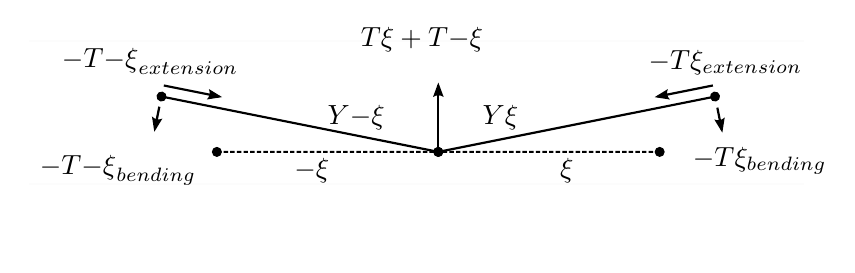
\begin{tikzpicture}[y=0.80pt, x=0.8pt,yscale=-1, inner sep=0pt, outer sep=0pt]
\begin{scope}[shift={(-16.10332,-55.70103)}]
  \begin{scope}[fill=black]
    \path[color=black,fill=black,line width=0.800pt] (101.0938,106.6875) --
      (103.0938,106.6875) -- (103.0938,105.6875) -- (101.0938,105.6875) --
      cycle(104.0938,106.6875) -- (106.0938,106.6875) -- (106.0938,105.6875) --
      (104.0938,105.6875) -- cycle(107.0938,106.6875) -- (109.0938,106.6875) --
      (109.0938,105.6875) -- (107.0938,105.6875) -- cycle(110.0938,106.6875) --
      (112.0938,106.6875) -- (112.0938,105.6875) -- (110.0938,105.6875) --
      cycle(113.0938,106.6875) -- (115.0938,106.6875) -- (115.0938,105.6875) --
      (113.0938,105.6875) -- cycle(116.0938,106.6875) -- (118.0938,106.6875) --
      (118.0938,105.6875) -- (116.0938,105.6875) -- cycle(119.0938,106.6875) --
      (121.0938,106.6875) -- (121.0938,105.6875) -- (119.0938,105.6875) --
      cycle(122.0938,106.6875) -- (124.0938,106.6875) -- (124.0938,105.6875) --
      (122.0938,105.6875) -- cycle(125.0938,106.6875) -- (127.0938,106.6875) --
      (127.0938,105.6875) -- (125.0938,105.6875) -- cycle(128.0938,106.6875) --
      (130.0938,106.6875) -- (130.0938,105.6875) -- (128.0938,105.6875) --
      cycle(131.0938,106.6875) -- (133.0938,106.6875) -- (133.0938,105.6875) --
      (131.0938,105.6875) -- cycle(134.0938,106.6875) -- (136.0938,106.6875) --
      (136.0938,105.6875) -- (134.0938,105.6875) -- cycle(137.0938,106.6875) --
      (139.0938,106.6875) -- (139.0938,105.6875) -- (137.0938,105.6875) --
      cycle(140.0938,106.6875) -- (142.0938,106.6875) -- (142.0938,105.6875) --
      (140.0938,105.6875) -- cycle(143.0938,106.6875) -- (145.0938,106.6875) --
      (145.0938,105.6875) -- (143.0938,105.6875) -- cycle(146.0938,106.6875) --
      (148.0938,106.6875) -- (148.0938,105.6875) -- (146.0938,105.6875) --
      cycle(149.0938,106.6875) -- (151.0938,106.6875) -- (151.0938,105.6875) --
      (149.0938,105.6875) -- cycle(152.0938,106.6875) -- (154.0938,106.6875) --
      (154.0938,105.6875) -- (152.0938,105.6875) -- cycle(155.0938,106.6875) --
      (157.0938,106.6875) -- (157.0938,105.6875) -- (155.0938,105.6875) --
      cycle(158.0938,106.6875) -- (160.0938,106.6875) -- (160.0938,105.6875) --
      (158.0938,105.6875) -- cycle(161.0938,106.6875) -- (163.0938,106.6875) --
      (163.0938,105.6875) -- (161.0938,105.6875) -- cycle(164.0938,106.6875) --
      (166.0938,106.6875) -- (166.0938,105.6875) -- (164.0938,105.6875) --
      cycle(167.0938,106.6875) -- (169.0938,106.6875) -- (169.0938,105.6875) --
      (167.0938,105.6875) -- cycle(170.0938,106.6875) -- (172.0938,106.6875) --
      (172.0938,105.6875) -- (170.0938,105.6875) -- cycle(173.0938,106.6875) --
      (175.0938,106.6875) -- (175.0938,105.6875) -- (173.0938,105.6875) --
      cycle(176.0938,106.6875) -- (178.0938,106.6875) -- (178.0938,105.6875) --
      (176.0938,105.6875) -- cycle(179.0938,106.6875) -- (181.0938,106.6875) --
      (181.0938,105.6875) -- (179.0938,105.6875) -- cycle(182.0938,106.6875) --
      (184.0938,106.6875) -- (184.0938,105.6875) -- (182.0938,105.6875) --
      cycle(185.0938,106.6875) -- (187.0938,106.6875) -- (187.0938,105.6875) --
      (185.0938,105.6875) -- cycle(188.0938,106.6875) -- (190.0938,106.6875) --
      (190.0938,105.6875) -- (188.0938,105.6875) -- cycle(191.0938,106.6875) --
      (193.0938,106.6875) -- (193.0938,105.6875) -- (191.0938,105.6875) --
      cycle(194.0938,106.6875) -- (196.0938,106.6875) -- (196.0938,105.6875) --
      (194.0938,105.6875) -- cycle(197.0938,106.6875) -- (199.0938,106.6875) --
      (199.0938,105.6875) -- (197.0938,105.6875) -- cycle(200.0938,106.6875) --
      (201.0938,106.6875) -- (202.0938,106.6875) -- (202.0938,105.6875) --
      (201.0938,105.6875) -- (200.0938,105.6875) -- cycle(203.0938,106.6875) --
      (205.0938,106.6875) -- (205.0938,105.6875) -- (203.0938,105.6875) --
      cycle(206.0938,106.6875) -- (208.0938,106.6875) -- (208.0938,105.6875) --
      (206.0938,105.6875) -- cycle(209.0938,106.6875) -- (211.0938,106.6875) --
      (211.0938,105.6875) -- (209.0938,105.6875) -- cycle(212.0938,106.6875) --
      (214.0938,106.6875) -- (214.0938,105.6875) -- (212.0938,105.6875) --
      cycle(215.0938,106.6875) -- (217.0938,106.6875) -- (217.0938,105.6875) --
      (215.0938,105.6875) -- cycle(218.0938,106.6875) -- (220.0938,106.6875) --
      (220.0938,105.6875) -- (218.0938,105.6875) -- cycle(221.0938,106.6875) --
      (223.0938,106.6875) -- (223.0938,105.6875) -- (221.0938,105.6875) --
      cycle(224.0938,106.6875) -- (226.0938,106.6875) -- (226.0938,105.6875) --
      (224.0938,105.6875) -- cycle(227.0938,106.6875) -- (229.0938,106.6875) --
      (229.0938,105.6875) -- (227.0938,105.6875) -- cycle(230.0938,106.6875) --
      (232.0938,106.6875) -- (232.0938,105.6875) -- (230.0938,105.6875) --
      cycle(233.0938,106.6875) -- (235.0938,106.6875) -- (235.0938,105.6875) --
      (233.0938,105.6875) -- cycle(236.0938,106.6875) -- (238.0938,106.6875) --
      (238.0938,105.6875) -- (236.0938,105.6875) -- cycle(239.0938,106.6875) --
      (241.0938,106.6875) -- (241.0938,105.6875) -- (239.0938,105.6875) --
      cycle(242.0938,106.6875) -- (244.0938,106.6875) -- (244.0938,105.6875) --
      (242.0938,105.6875) -- cycle(245.0938,106.6875) -- (247.0938,106.6875) --
      (247.0938,105.6875) -- (245.0938,105.6875) -- cycle(248.0938,106.6875) --
      (250.0938,106.6875) -- (250.0938,105.6875) -- (248.0938,105.6875) --
      cycle(251.0938,106.6875) -- (253.0938,106.6875) -- (253.0938,105.6875) --
      (251.0938,105.6875) -- cycle(254.0938,106.6875) -- (256.0938,106.6875) --
      (256.0938,105.6875) -- (254.0938,105.6875) -- cycle(257.0938,106.6875) --
      (259.0938,106.6875) -- (259.0938,105.6875) -- (257.0938,105.6875) --
      cycle(260.0938,106.6875) -- (262.0938,106.6875) -- (262.0938,105.6875) --
      (260.0938,105.6875) -- cycle(263.0938,106.6875) -- (265.0938,106.6875) --
      (265.0938,105.6875) -- (263.0938,105.6875) -- cycle(266.0938,106.6875) --
      (268.0938,106.6875) -- (268.0938,105.6875) -- (266.0938,105.6875) --
      cycle(269.0938,106.6875) -- (271.0938,106.6875) -- (271.0938,105.6875) --
      (269.0938,105.6875) -- cycle(272.0938,106.6875) -- (274.0938,106.6875) --
      (274.0938,105.6875) -- (272.0938,105.6875) -- cycle(275.0938,106.6875) --
      (277.0938,106.6875) -- (277.0938,105.6875) -- (275.0938,105.6875) --
      cycle(278.0938,106.6875) -- (280.0938,106.6875) -- (280.0938,105.6875) --
      (278.0938,105.6875) -- cycle(281.0938,106.6875) -- (283.0938,106.6875) --
      (283.0938,105.6875) -- (281.0938,105.6875) -- cycle(284.0938,106.6875) --
      (286.0938,106.6875) -- (286.0938,105.6875) -- (284.0938,105.6875) --
      cycle(287.0938,106.6875) -- (289.0938,106.6875) -- (289.0938,105.6875) --
      (287.0938,105.6875) -- cycle(290.0938,106.6875) -- (292.0938,106.6875) --
      (292.0938,105.6875) -- (290.0938,105.6875) -- cycle(293.0938,106.6875) --
      (295.0938,106.6875) -- (295.0938,105.6875) -- (293.0938,105.6875) --
      cycle(296.0938,106.6875) -- (298.0938,106.6875) -- (298.0938,105.6875) --
      (296.0938,105.6875) -- cycle(299.0938,106.6875) -- (301.0938,106.6875) --
      (301.0938,105.6875) -- (299.0938,105.6875) -- cycle;
    \path[draw=black,fill=black,even odd rule,line width=0.400pt]
      (103.0633,106.2010) .. controls (103.0633,107.3050) and (102.1673,108.2010) ..
      (101.0633,108.2010) .. controls (99.9593,108.2010) and (99.0633,107.3050) ..
      (99.0633,106.2010) .. controls (99.0633,105.0970) and (99.9593,104.2010) ..
      (101.0633,104.2010) .. controls (102.1673,104.2010) and (103.0633,105.0970) ..
      (103.0633,106.2010) -- cycle;
    \path[draw=black,fill=black,even odd rule,line width=0.400pt]
      (203.0633,106.2010) .. controls (203.0633,107.3050) and (202.1673,108.2010) ..
      (201.0633,108.2010) .. controls (199.9593,108.2010) and (199.0633,107.3050) ..
      (199.0633,106.2010) .. controls (199.0633,105.0970) and (199.9593,104.2010) ..
      (201.0633,104.2010) .. controls (202.1673,104.2010) and (203.0633,105.0970) ..
      (203.0633,106.2010) -- cycle;
    \path[draw=black,fill=black,even odd rule,line width=0.400pt]
      (303.0633,106.2010) .. controls (303.0633,107.3050) and (302.1673,108.2010) ..
      (301.0633,108.2010) .. controls (299.9593,108.2010) and (299.0633,107.3050) ..
      (299.0633,106.2010) .. controls (299.0633,105.0970) and (299.9593,104.2010) ..
      (301.0633,104.2010) .. controls (302.1673,104.2010) and (303.0633,105.0970) ..
      (303.0633,106.2010) -- cycle;
  \end{scope}
  \begin{scope}[fill=black]
    \path[color=black,fill=black,line width=0.800pt] (76.1875,80.7188) --
      (76.0000,81.6875) -- (201.0000,106.6875) -- (201.0937,106.7187) --
      (201.1874,106.6875) -- (326.1874,81.6875) -- (326.0000,80.7188) --
      (201.0938,105.6875) -- (76.1875,80.7188) -- cycle;
    \path[draw=black,fill=black,even odd rule,line width=0.400pt] (78.0253,81.5854)
      .. controls (77.8087,82.6680) and (76.7544,83.3709) .. (75.6719,83.1544) ..
      controls (74.5893,82.9378) and (73.8864,81.8835) .. (74.1029,80.8010) ..
      controls (74.3194,79.7184) and (75.3738,79.0155) .. (76.4563,79.2320) ..
      controls (77.5389,79.4485) and (78.2418,80.5029) .. (78.0253,81.5854) --
      cycle;
    \path[draw=black,fill=black,even odd rule,line width=0.400pt]
      (203.0633,106.2010) .. controls (203.0633,107.3050) and (202.1673,108.2010) ..
      (201.0633,108.2010) .. controls (199.9593,108.2010) and (199.0633,107.3050) ..
      (199.0633,106.2010) .. controls (199.0633,105.0970) and (199.9593,104.2010) ..
      (201.0633,104.2010) .. controls (202.1673,104.2010) and (203.0633,105.0970) ..
      (203.0633,106.2010) -- cycle;
    \path[draw=black,fill=black,even odd rule,line width=0.400pt] (328.0253,80.8166)
      .. controls (328.2418,81.8992) and (327.5389,82.9535) .. (326.4563,83.1700) ..
      controls (325.3738,83.3866) and (324.3194,82.6837) .. (324.1029,81.6011) ..
      controls (323.8864,80.5186) and (324.5893,79.4642) .. (325.6719,79.2477) ..
      controls (326.7544,79.0312) and (327.8087,79.7341) .. (328.0253,80.8166) --
      cycle;
  \end{scope}
  \begin{scope}[fill=black]
    \path[color=black,fill=black,line width=0.800pt] (200.5938,76.1875) --
      (200.5938,106.1875) -- (201.5938,106.1875) -- (201.5938,76.1875) --
      (200.5938,76.1875) -- cycle;
    \path[fill=black,line join=round,even odd rule,line width=0.500pt]
      (198.6831,81.4322) -- (201.0937,74.8767) -- (203.5043,81.4322) .. controls
      (202.0811,80.3849) and (200.1339,80.3909) .. (198.6831,81.4322) -- cycle;
  \end{scope}
  \path[fill=black] (178.797,148.02312) node[above right] (text6246) {};
  \path[fill=black] (256.10333,120.20103) node[above right] (text6273)
    {$\boldsymbol{\xi}$};
  \path[fill=black] (136.10332,120.20103) node[above right] (text6277)
    {$\boldsymbol{-\xi}$};
  \path[fill=black] (296.10333,71.201035) node[above right] (text6285)
    {$-\vstate{T}{}{\boldsymbol{\xi}}_{extension}$};
  \path[shift={(71.10332,65.91978)},draw=black,opacity=0.010,line join=miter,line
    cap=butt,line width=0.800pt] (-55.0000,54.7812) -- (295.0000,54.7812);
  \path[fill=black] (316.10333,116.20103) node[above right] (text4473)
    {$-\vstate{T}{}{\boldsymbol{\xi}}_{bending}$};
  \begin{scope}[shift={(0,-64.5)},shift={(0,0)}]
    \path[shift={(71.10332,65.91978)},draw=black,opacity=0.010,line join=miter,line
      cap=butt,line width=0.800pt] (-55.0000,54.7812) -- (295.0000,54.7812);
  \end{scope}
  \path[fill=black] (166.10332,61.201035) node[above right] (text4726)
    {$\vstate{T}{}{\boldsymbol{\xi}}+\vstate{T}{}{\boldsymbol{-\xi}}$};
  \begin{scope}[fill=black]
    \path[color=black,fill=black,line width=0.800pt] (74.5625,85.6875) --
      (72.5625,95.6875) -- (73.5625,95.9062) -- (75.5625,85.9062) --
      (74.5625,85.6875) -- cycle;
    \path[fill=black,line join=round,even odd rule,line width=0.500pt]
      (76.4671,91.1458) -- (72.8177,97.1013) -- (71.7395,90.2003) .. controls
      (72.9297,91.5064) and (74.8403,91.8824) .. (76.4671,91.1458) -- cycle;
  \end{scope}
  \begin{scope}[fill=black]
    \path[color=black,fill=black,line width=0.800pt] (77.1875,75.7188) --
      (77.0000,76.6875) -- (102.0000,81.6875) -- (102.1875,80.7188) --
      (77.1875,75.7188) -- cycle;
    \path[fill=black,line join=round,even odd rule,line width=0.500pt]
      (97.4484,77.8019) -- (103.4039,81.4513) -- (96.5029,82.5295) .. controls
      (97.8090,81.3393) and (98.1849,79.4287) .. (97.4484,77.8019) -- cycle;
  \end{scope}
  \begin{scope}[fill=black]
    \path[color=black,fill=black,line width=0.800pt] (327.5938,86.0938) --
      (326.6250,86.3125) -- (328.6250,96.3125) -- (329.5938,96.0938) --
      (327.5938,86.0938) -- cycle;
    \path[fill=black,line join=round,even odd rule,line width=0.500pt]
      (330.4506,90.5968) -- (329.3725,97.4978) -- (325.7230,91.5423) .. controls
      (327.3240,92.2902) and (329.2322,91.9024) .. (330.4507,90.5968) -- cycle;
  \end{scope}
  \begin{scope}[fill=black]
    \path[color=black,fill=black,line width=0.800pt] (325.0000,75.7188) --
      (300.0000,80.7188) -- (300.1875,81.6875) -- (325.1875,76.6875) --
      (325.0000,75.7188) -- cycle;
    \path[fill=black,line join=round,even odd rule,line width=0.500pt]
      (305.7075,82.5484) -- (298.8066,81.4702) -- (304.7620,77.8207) .. controls
      (304.0142,79.4217) and (304.4020,81.3299) .. (305.7075,82.5484) -- cycle;
  \end{scope}
  \path[fill=black] (21.103317,121.20103) node[above right] (text4217)
    {$-\vstate{T}{}{\boldsymbol{-\xi}}_{bending}$};
  \path[fill=black] (31.103317,71.201035) node[above right] (text4221)
    {$-\vstate{T}{}{\boldsymbol{-\xi}}_{extension}$};
  \path[fill=black] (221.10332,96.201035) node[above right] (text4282)
    {$\vstate{Y}{}{\boldsymbol{\xi}}$};
  \path[fill=black] (151.10332,96.201035) node[above right] (text4286)
    {$\vstate{Y}{}{\boldsymbol{-\xi}}$};
\end{scope}

\end{tikzpicture}


  \caption{The Hybrid Model Combines Bending and Extension Components}
  \label{fig:hybridmodel}
\end{figure}
%
As the two sides are pulled apart, the magnitude of the extension force in each bond increases, and the magnitude of the bending force decreases.  At the same time, the angle at which the extension force acts decreases, and the angle of action for the bending force increases.  For small amounts of bending and reasonable stretches, increased tension in the direction of the bond pair results in increased restorative force.
\section{Extension to arbitrary Poisson ratio}
\label{sec:arbitrary}
Although many materials have Poisson ratios of \(\nu\approx \sfrac{1}{3}\), it is nonetheless desirable to extend the model to materials with arbitrary Poisson ratios.  For isotropic, linearly elastic models of solid materials, Silling et al.\ extended the peridynamic material model to arbitrary material parameters in \cite{silling2007peridynamic} by decomposing the deformation into isotropic and deviatoric components.  In the absence of plastic deformation, we need only find the difference between the strain energy of a deformed bond-based plate and the strain energy of an elastic plate with Poisson's ratio \(\nu \neq \sfrac{1}{3}\).  The difference is a function of the isotropic strain in two dimensions, \(\theta_2\)
%
\begin{align}
    W' &= \frac{G\;h}{2}\left(\frac{3\nu-1}{1-\nu}\right)\theta_2^2 \notag \\
%    \theta_2 &= \frac{2}{m}\left(\underline{\omega x}\right)\bullet\underline{e} \notag \\
    \theta_2 &= \frac{2}{m}\int_A \omega(\boldsymbol{\xi})|\boldsymbol{\xi}|(|\vstate{Y}{}{\boldsymbol{\xi}}|-|\boldsymbol{\xi}|)\;dA_{\boldsymbol{\xi}} \notag \\
%    W_\text{total} &= \frac{G\;h}{2}\left(\frac{3\nu-1}{1-\nu}\right)\theta_2^2 + \frac{4\;G\;h}{m}\left(\underline{\omega e}\right)\bullet\underline{e}\notag
    W_\text{total} &= \frac{G\;h}{2}\left(\frac{3\nu-1}{1-\nu}\right)\theta_2^2 + \frac{4\;G\;h}{m}\int_A \omega(\boldsymbol{\xi})(|\vstate{Y}{}{\boldsymbol{\xi}}|-|\boldsymbol{\xi}|)^2\;dA_{\boldsymbol{\xi}}\notag
\end{align}
%
This is to be expected because the bond-based model was calibrated to the shear strain energy, leaving discrepancies proportional to the isotropic strain energy that fall to 0 as Poisson's ratio approaches \(\nu = \sfrac{1}{3}\).

This decomposition method inspires a similar approach to our plate model. To perform the same extension for the plate model in bending, we find the error in the 1-parameter strain energy for \(\nu \neq \sfrac{1}{3}\)
%
\begin{align}
    W'=&\frac{G h^3}{12(1-\nu)} \left(\kappa_1^2+\kappa_2^2+2\nu\kappa_1\kappa_2+2(1-\nu)\kappa_3^2 \right)\notag\\
    &-\frac{G h^3}{12(1-\frac{1}{3})} \left(\kappa_1^2+\kappa_2^2+\frac{2}{3}\nu\kappa_1\kappa_2+2(1-\frac{1}{3})\kappa_3^2 \right) \notag \\
    W'=&2G \frac{h^3}{12}\frac{3\nu-1}{1-\nu} \left(\frac{\kappa_1+\kappa_2}{2}\right)^2.\notag
\end{align}
%
The discrepancy in energy is proportional to the square of average curvature, \(\frac{\kappa_1+\kappa_2}{2} = \bar{\kappa}\), which we will also refer to as the isotropic curvature.  The isotropic curvature can be envisioned as the portion of the deformation that resembles a hemispherical bowl.  A complete decomposition of bending energy into isotropic and deviatoric components as performed by Fischer in \cite{fischer1992bending} produces a far more complex model and is unnecessary at this time.  For a single bond pair we can represent the curvature vector along the bond pair as 
%
\begin{equation}
    \boldsymbol{\kappa} _{\hat{\boldsymbol{\xi}}} = \frac{\vstate{Y}{}{\boldsymbol{\xi}}+\vstate{Y}{}{\boldsymbol{-\xi}}}{|\boldsymbol{\xi}|^2}\notag
\end{equation}
%
For large rotations, we can define an average curvature vector \(\bar{\boldsymbol{\kappa}}\).
This leads us to model the average curvature as 
%
\begin{align}
    \bar{\boldsymbol{\kappa}} &= \frac{1}{m} \int_0^\delta \int_0^{2\pi}\omega(\xi)\frac{\vstate{Y}{}{\boldsymbol{\xi}}+\vstate{Y}{}{\boldsymbol{-\xi}}}{\xi^2} \xi {\rm d}\phi {\rm d}\xi ;\notag \\
    m &= \int_0^\delta \int_0^{2\pi}\omega(\xi)\xi {\rm d}\phi {\rm d}\xi. \notag
\end{align}
%
The weighting function \(\omega(\xi)\) performs the same function as in the previous section.
We can rewrite the energy discrepancy in terms of \(\bar{\boldsymbol{\kappa}}\).
%
\begin{equation}
    W'=2G\frac{h^3}{12}\frac{3\nu-1}{1-\nu}\bar{\boldsymbol{\kappa}}^2. \notag
\end{equation}
%
We can take the Fr\'{e}chet derivative (details in \ref{sec:frechet}) to produce a correction force vector state
%
\begin{equation}
    \vstate{T'}{}{\boldsymbol{\xi}}=\frac{8G}{m}\frac{h^3}{12}\frac{3\nu-1}{1-\nu}\frac{\omega(\boldsymbol{\xi})}{\xi^2} \bar{\boldsymbol{\kappa}},
    \label{eq:pressureState}
\end{equation}
%
that is not directly dependent on the deformation of a single bond pair.  Instead, \cref{eq:pressureState} represents a bond-length dependent ``pressure'' applied to every pair of bonds extending from a node.  This ``pressure'' is proportional to the curvature vector at that node.
A weighting function \(\omega(\boldsymbol{\xi}) = |\boldsymbol{\xi}|\) can ensure that the integral expression for force at a point is convergent.  This extra term that is dependent on the bending of all the pairs around a material point means that the extension is not properly a \textit{bond-pair} model.  Instead, it would be more accurate to call it a \textit{bond-multiple} model, in which the bond forces and energies are functions of the relationship between a family of bonds.  In either the continuous or discrete cases, this model extension requires the additional step of evaluating the isotropic curvature at each point, but the increased complexity of the extended model captures in the local limit the behavior of a two-parameter elastic material plate.
%
\chapter{Numerical Simulation}
\section{Discretized Bond Pair Beam}
Discretizing the bond-pair model is primarily matter of exchanging integrals for sums. 
%
\begin{align}
%\label{eq:discreteBeamw}
w(\boldsymbol{\xi}_i) &= \omega(\boldsymbol{\xi}_i)\alpha \left[1+\cos(\theta(\vstate{Y}{}{\boldsymbol{\xi}_i},\vstate{Y}{}{-\boldsymbol{\xi}_i})) \right] \notag \\
&\approx \omega(\boldsymbol{\xi}_i)\frac{\alpha}{2}\left(\frac{v(\mathbf{x}+\boldsymbol{\xi}_i)-2v(\mathbf{x})+v(\mathbf{x}-\boldsymbol{\xi}_i)}{\boldsymbol{\xi}_i}\right)^2 \notag
\end{align}
%
in which $\boldsymbol{\xi}_i$ is the $i^\textnormal{th}$ bond emanating from the point $\mathbf{x}$ to each of the $n$ points within distance $\delta$ of point $\mathbf{x}$.
%
\begin{align}
%\label{eq:discretebeam}
\alpha &= \frac{c\; \Delta x}{m} ;\; c= EI ;\; m=\sum_{i=1}^n \omega(\boldsymbol{\xi}_i)\boldsymbol{\xi}_i^2 \implies \nonumber \\
W&=\Delta x \sum_{i=1}^n \frac{EI}{2}\omega(\boldsymbol{\xi}_i)\left(\frac{v(\mathbf{x}+\boldsymbol{\xi}_i)-2v(\mathbf{x})+v(\mathbf{x}-\boldsymbol{\xi}_i)}{\boldsymbol{\xi}_i}\right)^2\notag
\end{align}
%
Discretization of the original model results in the equation of motion
\begin{align}
\rho(\mathbf{x})\mathbf{\ddot{u}}(\mathbf{x}) = \mathbf{f}(\mathbf{x})&+\sum_i \omega(\boldsymbol{\xi}_i)\left\{\frac{\alpha(\mathbf{x})}{|\mathbf{p}_i |}\frac{\mathbf{p}_i}{|\mathbf{p}_i |}\times \left[ \frac{\mathbf{p}_i}{|\mathbf{p}_i |}\times \frac{\mathbf{q}_i}{|\mathbf{q}_i |}\right] \right. \notag \\
& \left. -\frac{\alpha(\mathbf{x}+\boldsymbol{\xi}_i)}{|\mathbf{p}_i |}\frac{(-\mathbf{p}_i)}{|\mathbf{p}_i |}\times\left[\frac{(-\mathbf{p}_i)}{|\mathbf{p}_i |}\times \frac{\mathbf{r}_i}{|\mathbf{r}_i |} \right] \right\} 
\label{eq:discretebeamEoM}
\end{align}
with
\begin{align}
\mathbf{p}_i &= \boldsymbol{\xi}_i+\mathbf{u}(\mathbf{x}+\boldsymbol{\xi}_i)-\mathbf{u}(\mathbf{x});\notag\\
\mathbf{q}_i &= -\boldsymbol{\xi}_i+\mathbf{u}(\mathbf{x}-\boldsymbol{\xi}_i)-\mathbf{u}(\mathbf{x});\notag\\
\mathbf{r}_i &= \boldsymbol{\xi}_i+\mathbf{u}(\mathbf{x}+2\boldsymbol{\xi}_i)-\mathbf{u}(\mathbf{x}+\boldsymbol{\xi}_i).\notag
\end{align}
and for small displacements and rotations in a uniform beam,
\begin{align}
\rho(\mathbf{x})\ddot{v}(\mathbf{x}) = &f(\mathbf{x})\notag \\
+&\alpha \sum_i 2\omega(\xi_i)\left(\frac{v(\mathbf{x}-2 \boldsymbol{\xi}_i)-4v(\mathbf{x}- \boldsymbol{\xi}_i)+6v(\mathbf{x})-4v(\mathbf{x}+ \boldsymbol{\xi}_i)+v(\mathbf{x}+2 \boldsymbol{\xi}_i)}{ \boldsymbol{\xi}_i^2}\right) \notag
\end{align}
It is worth noting the similarity between this expression and a finite-difference fourth derivative of displacement, a result expected from Euler beam theory.
This discretization requires that nodes be evenly spaced along the entire beam, otherwise the displacement \(v(\mathbf{x}- \boldsymbol{\xi}_i)\) is ill-defined. 
For this reason, the discretization does not allow for areas of higher and lower ``resolution''. 

\section{Discretized Bond Pair Plate}

%
\begin{figure}[h]
  \centering
\resizebox{.7\linewidth}{!}{\subinputfrom{\diagrampath}{discretePlate.eps_tex}}
\caption{Discretized peridynamic plate with illustrated bond pair}
\label{fig:discretePlate}
\end{figure}
%
As with the beam, discretizing the bond-pair model is primarily matter of exchanging integrals for sums. 
%
%\begin{align}
%w(\boldsymbol{\xi}_i) &= \omega(\boldsymbol{\xi}_i)\alpha \left[1+\cos(\theta(\vstate{Y}{}{\boldsymbol{\xi}_i},\vstate{Y}{}{-\boldsymbol{\xi}_i})) \right] \notag \\
%&\approx \omega(\boldsymbol{\xi}_i)\frac{\alpha}{2}\left(\frac{z(\mathbf{x}+\boldsymbol{\xi}_i)-2z(\mathbf{x})+z(\mathbf{x}-\boldsymbol{\xi}_i)}{\boldsymbol{\xi}_i}\right)^2 \notag
%\end{align}
%%
%in which $\boldsymbol{\xi}_i$ is the $i^\textnormal{th}$ bond emanating from the point $\mathbf{x}$ to each of the $n$ points within distance $\delta$ of point $\mathbf{x}$.
%
\begin{align}
    \alpha &= \frac{c\; (\Delta x)^2}{m} ;\; c= \frac{G}{(1-\nu)}\frac{h^3}{12};\; m=\sum_{i=1}^n \omega(\boldsymbol{\xi}_i)\boldsymbol{\xi}_i^2 \implies \nonumber \\
    W&=(\Delta x)^2 \sum_{i=1}^n \omega(\boldsymbol{\xi}_i)\frac{G}{2(1-\nu)}\frac{h^3}{12}\left(\frac{z(\mathbf{x}+\boldsymbol{\xi}_i)-2z(\mathbf{x})+z(\mathbf{x}-\boldsymbol{\xi}_i)}{|\boldsymbol{\xi}_i|}\right)^2 \notag
\end{align}
%
Discretization of the 1-parameter bending model results in the same equation of motion as for the beam model (eq. \ref{eq:discretebeamEoM}).
%
%\begin{align}
%    \label{eq:discreteEoM}
%    \rho(\mathbf{x})\mathbf{\ddot{u}}(\mathbf{x}) = \mathbf{f}(\mathbf{x})&+\sum_i \omega(\boldsymbol{\xi}_i)\left\{\frac{\alpha(\mathbf{x})}{|\mathbf{p}_i |}\frac{\mathbf{p}_i}{|\mathbf{p}_i |}\times \left[ \frac{\mathbf{p}_i}{|\mathbf{p}_i |}\times \frac{\mathbf{q}_i}{|\mathbf{q}_i |}\right] \right.  \\
%    & \left. -\frac{\alpha(\mathbf{x}+\boldsymbol{\xi}_i)}{|\mathbf{p}_i |}\frac{(-\mathbf{p}_i)}{|\mathbf{p}_i |}\times\left[\frac{(-\mathbf{p}_i)}{|\mathbf{p}_i |}\times \frac{\mathbf{r}_i}{|\mathbf{r}_i |} \right] \right\} \notag
%\end{align}
%with
%\begin{align}
%    \mathbf{p}_i &= \boldsymbol{\xi}_i+\mathbf{u}(\mathbf{x}+\boldsymbol{\xi}_i)-\mathbf{u}(\mathbf{x});\notag\\
%    \mathbf{q}_i &= -\boldsymbol{\xi}_i+\mathbf{u}(\mathbf{x}-\boldsymbol{\xi}_i)-\mathbf{u}(\mathbf{x});\notag\\
%    \mathbf{r}_i &= \boldsymbol{\xi}_i+\mathbf{u}(\mathbf{x}+2\boldsymbol{\xi}_i)-\mathbf{u}(\mathbf{x}+\boldsymbol{\xi}_i).\notag
%\end{align}
%

Implementing the 2-parameter model requires finding the isotropic curvature at each point.
%
\begin{align*}
    \bar{\boldsymbol{\kappa}}(\mathbf{x}) &= \frac{1}{m} \sum_i \omega(\boldsymbol{\xi}_i)\frac{\mathbf{p}_i +\mathbf{q}_i }{\boldsymbol{\xi}_i^2};\notag \\
    m(\mathbf{x})  &= \sum_i \omega(\boldsymbol{\xi}_i); \notag \\
    \alpha^\text{iso}(\mathbf{x}) &= \frac{4G}{m}\frac{h^3}{12}\frac{3\nu-1}{1-\nu}(\Delta x)^2;\\
    f^\text{iso}(\mathbf{x}) &= \sum_j \left\{\left[\alpha^\text{iso}(\mathbf{x})\bar{\boldsymbol{\kappa}}(\mathbf{x})-\alpha^\text{iso}(\mathbf{x}+\boldsymbol{\xi}_j)\bar{\boldsymbol{\kappa}}(\mathbf{x}+\boldsymbol{\xi}_j) \right] \frac{\omega(\boldsymbol{\xi}_j)}{\boldsymbol{\xi}_j^2} \right\}
\end{align*}
%
As with the discretized beam, the discretization of the bond-pair plate (\cref{fig:discretePlate}) must be absolutely regular. 
Discretizing the bond-pair model as proposed above requires that nodes be evenly spaced, $\Delta x$, throughout the entire plate, otherwise the displacement \(z(\mathbf{x}-\boldsymbol{\xi}_i)\) is undefined.  For this reason, the discretization does not allow for areas of higher and lower ``resolution''.  This restriction, while inconvenient in the 1D case, is fairly restricting for plate analysis. An extension to this discretization that would allow changing mesh resolution will require interpolation between the nodes.  
%
%
%
%
%\begin{figure}[tbp]
%  \centering
%  \input{\diagrampath/VirtualPoint.tex}
%  \caption{Virtual Points Pair Up Unpaired Neighbors}
%  \label{fig:virtualpoint}
%\end{figure}
%
%
%\section{Bond Multiple Material Model}
%The requirement for a perfectly regular discretization makes the bond pair model difficult to use for many problems. 
%One proposed solution to this shortcoming is the \textit{bond-multiple} material model. 
%In a bond-multiple material, there exists a bond-pair potential energy for \textit{every possible combination of 2 bonds} emanating from a material point
%%
%\begin{equation}
%\label{eq:bondMultiple}
%W=\int_{\mathcal{H}} \int_{\mathcal{H}}  \omega(\boldsymbol{\xi})\omega(\boldsymbol{\zeta})w(\vstate{Y}{}{\boldsymbol{\xi}},\vstate{Y}{}{\boldsymbol{\zeta}})d\boldsymbol{\zeta} d \boldsymbol{\xi} .
%\end{equation}
%%
%The bond-pair energy expression assumes bonds that are antiparallel in the undeformed configuration. 
%To incorporate the energy of bonds that are collinear or otherwise oriented in the undeformed configuration, we modify the bond-pair energy expression as shown in \cref{eq:bondMultw}.
%%
%\begin{equation}
%\label{eq:bondMultw}
%w(\vstate{Y}{}{\boldsymbol{\xi}},\vstate{Y}{}{\boldsymbol{\zeta}})= \alpha [1-\cos \left(\theta(\vstate{Y}{}{\boldsymbol{\xi}},\vstate{Y}{}{\boldsymbol{\zeta}})-\theta( \boldsymbol{\xi} , \boldsymbol{\zeta} )\right) ] d\boldsymbol{\zeta} d \boldsymbol{\xi} 
%\end{equation}
%%
%\section{Bond Multiple Beam}
%For the beam model, this transforms the expression for strain energy density into
%%
%\begin{equation}
%\label{eq:bondMultipleBeam}
%W=\int_{-\delta}^{\delta} \int_{-\delta}^{\delta} \omega(\xi)\omega(\zeta) \alpha[1-\cos \left(\theta(\vstate{Y}{}{\xi},\vstate{Y}{}{\zeta})-\theta( \xi , \zeta )\right) ] d\zeta d \xi .
%\end{equation}
%
%As with the bond pair model, by making the simplifying assumptions of beam length, displacement, and rotation, the strain energy density of the bond multiple beam can be shown to equal that of a classical Euler beam in bending. 
%This analysis benefits greatly from the fact that the undeformed angle between the bonds in \cref{fig:bondMultipleA,fig:bondMultipleB} is either \(0\) or \(\pi\).
%%
%\begin{figure}[h]
%  \centering
%\subinputfrom{\diagrampath}{bondMultiple.eps_tex}
%\caption{Bonds initially antiparallel}
%\label{fig:bondMultipleA}
%\end{figure}
%%
%\begin{figure}[h]
%  \centering
%\subinputfrom{\diagrampath}{bondMultiple2.eps_tex}
%\caption{Bonds initially collinear}
%\label{fig:bondMultipleB}
%\end{figure}
%%
%That is to say, all bonds run along the same beam, and so are initially collinear or antiparallel.
%%
%\begin{align}
%\label{eq:bondMultipleBeamS}
%W&= \alpha\int_{-\delta}^{\delta}  \omega(\xi) \int_{-\delta}^{\delta} \omega(\zeta) [1-\cos \left(\theta(\vstate{Y}{}{\xi},\vstate{Y}{}{\zeta})-\theta( \xi , \zeta )\right) ]  d\zeta d \xi \notag\\
%W&= \alpha\int_{-\delta}^{\delta} \omega(\xi) \int_{-\delta}^{\delta} \omega(\zeta) [1-\frac{\xi}{|\xi|}\frac{\zeta}{|\zeta|}\cos \left(\theta(\vstate{Y}{}{\xi},\vstate{Y}{}{\zeta})\right) ] d\zeta d \xi \notag\\
%W&\approx \alpha\int_{-\delta}^{\delta} \omega(\xi) \int_{-\delta}^{\delta} \omega(\zeta) \frac{1}{2}\left(\frac{y(x+\xi)-y(x)}{\xi}-\frac{y(x+\zeta)-y(x)}{\zeta}\right)^2 d\zeta d \xi \notag\\
%W&\approx \alpha\int_{-\delta}^{\delta} \omega(\xi) \int_{-\delta}^{\delta} \omega(\zeta) \frac{1}{2}\left(\frac{\partial^2 y}{\partial x^2}\right)^2\left(\xi-\zeta\right)^2 d\zeta d \xi \notag\\
%\end{align}
%%
%Again, by choosing our coefficients, we retrieve the strain energy density of the Euler beam.
%%
%\begin{align}
%\label{eq:classicMultiBeam}
%\alpha = \frac{c}{m} ;\; c= EI ;\; m=\int_{-\delta}^\delta \int_{-\delta}^\delta \omega(\xi)\omega(\zeta)\left(\xi-\zeta\right)^2 d\zeta d\xi \implies W\approx\frac{EI}{2}\left(\frac{\partial^2 y}{\partial x^2}\right)^2 
%\end{align}
%%
%The major advantage of this bond-multiple model lies in the discretization. 
%Because the two bond vectors are independent of each other, there is no need to require that node spacing be perfectly regular.
%%
%\section{Bond Multiple Plate}
%
%Analysis of a bond multiple plate is much more complex. 
%Unlike the previous analyses, the undeformed bond pairs can have any angle. 
%This means that transverse displacement of a point will result in increased bond angle for some bonds, decreased bond angle for others, and no change for orthogonal bonds. 
%It is difficult to formulate an integrable expression for the change in bond-pair angle for bonds initially separated by an arbitrary angle.
%
%For the bond-multiple beam, it was possible to find a polynomial expression for \(\theta\) and for \(\Delta\theta\) of the deformed pairs by expanding the series for sine and cosine around \(\theta\) at \(0\) and at \(\pi\), but this isn't possible when some undeformed bonds have an angle of \(\frac{\pi}{2}\) or any other angle. 
%
%Additionally, numerical integration of a plate deformed in cylindrical bending (\(\kappa_{11}\) only) with \(w=\sin^2(\theta)\) indicates a cubic relationship between curvature and strain energy density, not the quadratic relationship we are looking for. 
%For very small bending, we can expect the same result from \(w=1-\cos(\theta)\).
%
%More exotic energy functions may be possible.
%For example, the bond-multiple energy function:
%%
%\begin{equation}
%w=|\cos (\theta(\vstate{Y}{}{\xi},\vstate{Y}{}{\zeta}))-\cos(\theta( \xi , \zeta ))|
% \end{equation}
%%
%results in strain energy that is quadratic in \(\kappa_{11}\) for small cylindrical curvature, but has not been verified for other curvature types. 
%Additionally, this energy function is physically nonintuitive.
\subsection{Curved Shapes}
On a curved surface, the location of the point $\mathbf{x} - \boldsymbol{\xi}$ might be off of the surface entirely.
One method of applying the bond-pair model to curved surfaces is through the use of ``virtual'' points.
These points have no mass and do not have families of peridynamic neighbors, they only allow the definition of bond pairs that are straight in the undeformed configuration.
%
\begin{figure}[tbp]
  \centering
  
\definecolor{cffffff}{RGB}{255,255,255}


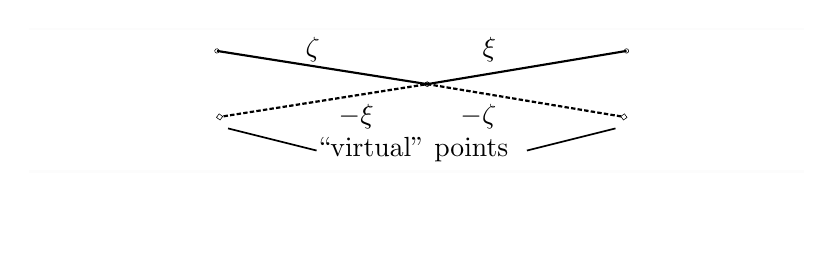
\begin{tikzpicture}[y=0.80pt, x=0.8pt,yscale=-1, inner sep=0pt, outer sep=0pt]
\begin{scope}[shift={(-16.10332,-55.70103)}]
    \path[color=black,fill=black,line width=0.800pt] (196.0312,80.7188) --
      (195.8438,80.7500) -- (196.0000,81.7188) -- (196.0938,81.6875) --
      (197.8125,82.0000) -- (197.9688,81.0000) -- (196.1875,80.7188) --
      (196.0938,80.6875) -- cycle(192.8750,81.1875) -- (193.0312,82.1875) --
      (195.0312,81.8750) -- (194.8750,80.9062) -- cycle(198.8125,82.1562) --
      (200.7812,82.5000) -- (200.9375,81.5000) -- (198.9688,81.1875) --
      cycle(189.9375,81.6562) -- (190.0938,82.6562) -- (192.0625,82.3438) --
      (191.9062,81.3438) -- cycle(201.7500,82.6562) -- (203.7500,82.9688) --
      (203.9062,82.0000) -- (201.9375,81.6562) -- cycle(186.9688,82.1250) --
      (187.1250,83.1250) -- (189.0938,82.8125) -- (188.9375,81.8125) --
      cycle(204.7188,83.1562) -- (206.6875,83.4688) -- (206.8750,82.5000) --
      (204.8750,82.1562) -- cycle(184.0000,82.5938) -- (184.1562,83.5938) --
      (186.1250,83.2812) -- (185.9688,82.2812) -- cycle(207.6875,83.6250) --
      (209.6562,83.9688) -- (209.8125,82.9688) -- (207.8438,82.6562) --
      cycle(181.0312,83.0625) -- (181.1875,84.0625) -- (183.1562,83.7500) --
      (183.0000,82.7500) -- cycle(210.6562,84.1250) -- (212.6250,84.4688) --
      (212.7812,83.4688) -- (210.8125,83.1562) -- cycle(178.0625,83.5312) --
      (178.2188,84.5312) -- (180.1875,84.2188) -- (180.0312,83.2188) --
      cycle(213.5938,84.6250) -- (215.5625,84.9688) -- (215.7500,83.9688) --
      (213.7812,83.6250) -- cycle(175.0938,84.0000) -- (175.2500,85.0000) --
      (177.2500,84.6875) -- (177.0938,83.6875) -- cycle(216.5625,85.1250) --
      (218.5312,85.4375) -- (218.6875,84.4688) -- (216.7188,84.1250) --
      cycle(172.1562,84.4688) -- (172.3125,85.4688) -- (174.2812,85.1562) --
      (174.1250,84.1562) -- cycle(169.1875,84.9375) -- (169.3438,85.9375) --
      (171.3125,85.6250) -- (171.1562,84.6250) -- cycle(219.5312,85.6250) --
      (221.5000,85.9375) -- (221.6562,84.9688) -- (219.6875,84.6250) --
      cycle(166.2188,85.4062) -- (166.3750,86.4062) -- (168.3438,86.0938) --
      (168.1875,85.0938) -- cycle(222.4688,86.0938) -- (224.4375,86.4375) --
      (224.6250,85.4375) -- (222.6562,85.1250) -- cycle(163.2500,85.8750) --
      (163.4062,86.8750) -- (165.3750,86.5625) -- (165.2188,85.5625) --
      cycle(225.4375,86.5938) -- (227.4062,86.9375) -- (227.5625,85.9375) --
      (225.5938,85.6250) -- cycle(160.2812,86.3438) -- (160.4375,87.3438) --
      (162.4375,87.0312) -- (162.2812,86.0312) -- cycle(228.4062,87.0938) --
      (230.3750,87.4062) -- (230.5312,86.4375) -- (228.5625,86.0938) --
      cycle(157.3125,86.8125) -- (157.4688,87.8125) -- (159.4688,87.5000) --
      (159.3125,86.5000) -- cycle(231.3438,87.5938) -- (233.3438,87.9062) --
      (233.5000,86.9375) -- (231.5312,86.5938) -- cycle(154.3750,87.2812) --
      (154.5312,88.2812) -- (156.5000,87.9688) -- (156.3438,86.9688) --
      cycle(234.3125,88.0625) -- (236.2812,88.4062) -- (236.4688,87.4062) --
      (234.4688,87.0938) -- cycle(151.4062,87.7500) -- (151.5625,88.7500) --
      (153.5312,88.4375) -- (153.3750,87.4375) -- cycle(237.2812,88.5625) --
      (239.2500,88.9062) -- (239.4062,87.9062) -- (237.4375,87.5938) --
      cycle(148.4375,88.2188) -- (148.5938,89.2188) -- (150.5625,88.9062) --
      (150.4062,87.9062) -- cycle(240.2188,89.0625) -- (242.2188,89.4062) --
      (242.3750,88.4062) -- (240.4062,88.0625) -- cycle(145.4688,88.6875) --
      (145.6250,89.6875) -- (147.5938,89.3750) -- (147.4375,88.3750) --
      cycle(243.1875,89.5625) -- (245.1562,89.8750) -- (245.3438,88.9062) --
      (243.3438,88.5625) -- cycle(142.5000,89.1562) -- (142.6562,90.1562) --
      (144.6562,89.8438) -- (144.5000,88.8438) -- cycle(246.1562,90.0625) --
      (248.1250,90.3750) -- (248.2812,89.4062) -- (246.3125,89.0625) --
      cycle(139.5625,89.6250) -- (139.7188,90.6250) -- (141.6875,90.3125) --
      (141.5312,89.3125) -- cycle(249.1250,90.5312) -- (251.0938,90.8750) --
      (251.2500,89.8750) -- (249.2812,89.5625) -- cycle(136.5938,90.0938) --
      (136.7500,91.0938) -- (138.7188,90.7812) -- (138.5625,89.7812) --
      cycle(252.0625,91.0312) -- (254.0312,91.3750) -- (254.2188,90.3750) --
      (252.2500,90.0625) -- cycle(133.6250,90.5625) -- (133.7812,91.5625) --
      (135.7500,91.2500) -- (135.5938,90.2500) -- cycle(255.0312,91.5312) --
      (257.0000,91.8438) -- (257.1562,90.8750) -- (255.1875,90.5312) --
      cycle(130.6562,91.0312) -- (130.8125,92.0312) -- (132.7812,91.7188) --
      (132.6250,90.7188) -- cycle(258.0000,92.0312) -- (259.9688,92.3438) --
      (260.1250,91.3750) -- (258.1562,91.0312) -- cycle(127.6875,91.5000) --
      (127.8438,92.4688) -- (129.8125,92.1875) -- (129.6562,91.1875) --
      cycle(260.9375,92.5000) -- (262.9062,92.8438) -- (263.0938,91.8438) --
      (261.1250,91.5312) -- cycle(124.7188,91.9688) -- (124.8750,92.9375) --
      (126.8750,92.6250) -- (126.7188,91.6562) -- cycle(263.9062,93.0000) --
      (265.8750,93.3438) -- (266.0312,92.3438) -- (264.0625,92.0312) --
      cycle(121.7812,92.4375) -- (121.9375,93.4062) -- (123.9062,93.0938) --
      (123.7500,92.1250) -- cycle(266.8750,93.5000) -- (268.8438,93.8438) --
      (269.0000,92.8438) -- (267.0312,92.5000) -- cycle(118.8125,92.9062) --
      (118.9688,93.8750) -- (120.9375,93.5625) -- (120.7812,92.5938) --
      cycle(269.8125,94.0000) -- (271.8125,94.3125) -- (271.9688,93.3438) --
      (270.0000,93.0000) -- cycle(115.8438,93.3750) -- (116.0000,94.3438) --
      (117.9688,94.0312) -- (117.8125,93.0625) -- cycle(272.7812,94.5000) --
      (274.7500,94.8125) -- (274.9375,93.8438) -- (272.9375,93.5000) --
      cycle(112.8750,93.8438) -- (113.0312,94.8125) -- (115.0000,94.5000) --
      (114.8438,93.5312) -- cycle(109.9062,94.3125) -- (110.0625,95.2812) --
      (112.0312,94.9688) -- (111.9062,94.0000) -- cycle(275.7500,94.9688) --
      (277.7188,95.3125) -- (277.8750,94.3125) -- (275.9062,94.0000) --
      cycle(106.9375,94.7812) -- (107.0938,95.7500) -- (109.0938,95.4375) --
      (108.9375,94.4688) -- cycle(278.7188,95.4688) -- (280.6875,95.8125) --
      (280.8438,94.8125) -- (278.8750,94.5000) -- cycle(104.0000,95.2500) --
      (104.1562,96.2188) -- (106.1250,95.9062) -- (105.9688,94.9375) --
      cycle(281.6562,95.9688) -- (283.6250,96.2812) -- (283.8125,95.3125) --
      (281.8125,94.9688) -- cycle(101.0312,95.7188) -- (101.1875,96.6875) --
      (103.1562,96.3750) -- (103.0000,95.4062) -- cycle(284.6250,96.4688) --
      (286.0312,96.6875) -- (286.1875,95.7188) -- (284.7812,95.4688) -- cycle;
    \path[draw=black,fill=cffffff,even odd rule,line width=0.200pt]
      (102.0681,94.6170) -- (100.8917,96.2344) -- (102.5092,97.4108) --
      (103.6855,95.7933) -- (102.0681,94.6170) -- cycle;
    \path[draw=black,even odd rule,line width=0.200pt] (197.0833,81.2052) ..
      controls (197.0813,81.7572) and (196.6310,82.2033) .. (196.0791,82.2009) ..
      controls (195.5271,82.1985) and (195.0810,81.7487) .. (195.0833,81.1967) ..
      controls (195.0853,80.6447) and (195.5356,80.1986) .. (196.0876,80.2010) ..
      controls (196.6396,80.2034) and (197.0857,80.6532) .. (197.0833,81.2052) --
      cycle;
    \path[draw=black,fill=cffffff,even odd rule,line width=0.200pt]
      (285.1521,94.6088) -- (283.5247,95.7713) -- (284.6871,97.3987) --
      (286.3146,96.2362) -- (285.1521,94.6088) -- cycle;
    \path[color=black,fill=black,line width=0.800pt] (101.1875,65.7188) --
      (101.0312,66.6875) -- (196.0312,81.6875) -- (196.0938,81.7188) --
      (196.1875,81.6875) -- (286.1875,66.6875) -- (286.0312,65.7188) --
      (196.0937,80.7188) -- (101.1875,65.7188) -- cycle;
    \path[draw=black,even odd rule,line width=0.200pt] (102.0713,66.3539) ..
      controls (101.9852,66.8991) and (101.4729,67.2718) .. (100.9276,67.1857) ..
      controls (100.3824,67.0996) and (100.0097,66.5872) .. (100.0958,66.0420) ..
      controls (100.1819,65.4967) and (100.6943,65.1241) .. (101.2395,65.2102) ..
      controls (101.7848,65.2962) and (102.1574,65.8086) .. (102.0713,66.3539) --
      cycle;
    \path[draw=black,even odd rule,line width=0.200pt] (197.0833,81.1968) ..
      controls (197.0853,81.7488) and (196.6396,82.1988) .. (196.0876,82.2011) ..
      controls (195.5356,82.2035) and (195.0857,81.7574) .. (195.0833,81.2054) ..
      controls (195.0813,80.6534) and (195.5271,80.2035) .. (196.0791,80.2011) ..
      controls (196.6310,80.1987) and (197.0810,80.6449) .. (197.0833,81.1968) --
      cycle;
    \path[draw=black,even odd rule,line width=0.200pt] (287.0700,66.0399) ..
      controls (287.1607,66.5844) and (286.7925,67.1000) .. (286.2480,67.1907) ..
      controls (285.7035,67.2815) and (285.1880,66.9132) .. (285.0972,66.3687) ..
      controls (285.0064,65.8242) and (285.3747,65.3087) .. (285.9192,65.2179) ..
      controls (286.4637,65.1272) and (286.9792,65.4954) .. (287.0700,66.0399) --
      cycle;
  \path[fill=black] (178.797,148.02312) node[above right] (text6246) {};
  \path[fill=black] (221.10332,71.201035) node[above right] (text6273)
    {$\boldsymbol{\xi}$};
  \path[fill=black] (156.10332,101.20103) node[above right] (text6277)
    {$\boldsymbol{-\xi}$};
  \path[shift={(71.10332,65.91978)},draw=black,opacity=0.010,line join=miter,line
    cap=butt,line width=0.800pt] (-55.0000,54.7812) -- (295.0000,54.7812);
  \begin{scope}[shift={(0,-64.5)},shift={(0,0)}]
    \path[shift={(71.10332,65.91978)},draw=black,opacity=0.010,line join=miter,line
      cap=butt,line width=0.800pt] (-55.0000,54.7812) -- (295.0000,54.7812);
  \end{scope}
  \path[fill=black] (141.10332,71.201035) node[above right] (text5341)
    {$\boldsymbol{\zeta}$};
  \path[fill=black] (211.10332,101.20103) node[above right] (text5345)
    {$\boldsymbol{-\zeta}$};
  \path[fill=black] (146.10332,116.20103) node[above right] (text5751)
    {``virtual'' points};
    \path[color=black,fill=black,line width=0.640pt] (106.1971,100.8260) --
      (106.0096,101.5760) -- (146.0096,111.5760) -- (146.1971,110.8260) --
      (106.1971,100.8260) -- cycle;
    \path[line join=round,even odd rule,line width=0.500pt] (107.3630,102.5138) --
      (105.0529,100.9424) -- (107.8307,100.6429) .. controls (107.2862,101.0936) and
      (107.0997,101.8498) .. (107.3630,102.5138) -- cycle;
    \path[color=black,fill=black,line width=0.640pt] (281.0096,100.8260) --
      (241.0096,110.8260) -- (241.1971,111.5760) -- (281.1971,101.5760) --
      (281.0096,100.8260) -- cycle;
    \path[line join=round,even odd rule,line width=0.500pt] (279.3741,100.6355) --
      (282.1518,100.9349) -- (279.8418,102.5064) .. controls (280.1101,101.8525) and
      (279.9189,101.0974) .. (279.3740,100.6355) -- cycle;
\end{scope}

\end{tikzpicture}


  \caption{Virtual Points Allow Straight Pairs on Curved Surfaces}
  \label{fig:virtualPair}
\end{figure}
%
In the simplest method, each virtual point is located just above or below a real point in the model.
In this case, properties such as displacement are taken to be the same as for the nearby real point.
%
\begin{figure}[tbp]
  \centering
  
\definecolor{cffffff}{RGB}{255,255,255}


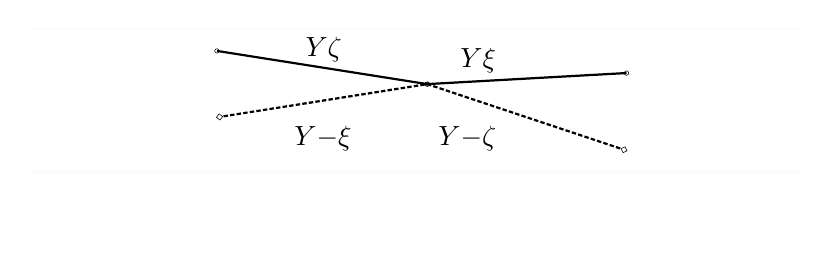
\begin{tikzpicture}[y=0.80pt, x=0.8pt,yscale=-1, inner sep=0pt, outer sep=0pt]
\begin{scope}[shift={(-16.10332,-55.70103)}]
    \path[color=black,fill=black,line width=0.800pt] (196.0312,80.7188) --
      (195.8438,80.7500) -- (195.9688,81.5625) -- (195.9375,81.6875) --
      (196.0000,81.7188) -- (196.0312,81.7188) -- (197.6875,82.2500) --
      (198.0000,81.3125) -- (196.2500,80.7188) -- (196.1563,80.6875) --
      cycle(192.8750,81.1875) -- (193.0312,82.1875) -- (195.0312,81.8750) --
      (194.8750,80.9062) -- cycle(189.9375,81.6562) -- (190.0938,82.6562) --
      (192.0625,82.3438) -- (191.9062,81.3438) -- cycle(198.6250,82.5625) --
      (200.5312,83.1875) -- (200.8438,82.2500) -- (198.9375,81.6250) --
      cycle(186.9688,82.1250) -- (187.1250,83.1250) -- (189.0938,82.8125) --
      (188.9375,81.8125) -- cycle(184.0000,82.5938) -- (184.1562,83.5938) --
      (186.1250,83.2812) -- (185.9688,82.2812) -- cycle(201.4688,83.5312) --
      (203.3750,84.1562) -- (203.6875,83.1875) -- (201.7812,82.5625) --
      cycle(181.0312,83.0625) -- (181.1875,84.0625) -- (183.1562,83.7500) --
      (183.0000,82.7500) -- cycle(178.0625,83.5312) -- (178.2188,84.5312) --
      (180.1875,84.2188) -- (180.0312,83.2188) -- cycle(204.3125,84.4688) --
      (206.2188,85.0938) -- (206.5312,84.1562) -- (204.6250,83.5312) --
      cycle(175.0938,84.0000) -- (175.2500,85.0000) -- (177.2500,84.6875) --
      (177.0938,83.6875) -- cycle(172.1562,84.4688) -- (172.3125,85.4688) --
      (174.2812,85.1562) -- (174.1250,84.1562) -- cycle(207.1562,85.4062) --
      (209.0625,86.0312) -- (209.3750,85.0938) -- (207.4688,84.4688) --
      cycle(169.1875,84.9375) -- (169.3438,85.9375) -- (171.3125,85.6250) --
      (171.1562,84.6250) -- cycle(166.2188,85.4062) -- (166.3750,86.4062) --
      (168.3438,86.0938) -- (168.1875,85.0938) -- cycle(210.0000,86.3750) --
      (211.9062,87.0000) -- (212.2188,86.0312) -- (210.3125,85.4062) --
      cycle(163.2500,85.8750) -- (163.4062,86.8750) -- (165.3750,86.5625) --
      (165.2188,85.5625) -- cycle(160.2812,86.3438) -- (160.4375,87.3438) --
      (162.4375,87.0312) -- (162.2812,86.0312) -- cycle(212.8438,87.3125) --
      (214.7500,87.9375) -- (215.0625,87.0000) -- (213.1562,86.3750) --
      cycle(157.3125,86.8125) -- (157.4688,87.8125) -- (159.4688,87.5000) --
      (159.3125,86.5000) -- cycle(154.3750,87.2812) -- (154.5312,88.2812) --
      (156.5000,87.9688) -- (156.3438,86.9688) -- cycle(215.6875,88.2500) --
      (217.5938,88.9062) -- (217.9062,87.9375) -- (216.0312,87.3125) --
      cycle(151.4062,87.7500) -- (151.5625,88.7500) -- (153.5312,88.4375) --
      (153.3750,87.4375) -- cycle(148.4375,88.2188) -- (148.5938,89.2188) --
      (150.5625,88.9062) -- (150.4062,87.9062) -- cycle(218.5312,89.2188) --
      (220.4375,89.8438) -- (220.7500,88.9062) -- (218.8750,88.2500) --
      cycle(145.4688,88.6875) -- (145.6250,89.6875) -- (147.5938,89.3750) --
      (147.4375,88.3750) -- cycle(142.5000,89.1562) -- (142.6562,90.1562) --
      (144.6562,89.8438) -- (144.5000,88.8438) -- cycle(221.4062,90.1562) --
      (223.2812,90.7812) -- (223.5938,89.8438) -- (221.7188,89.2188) --
      cycle(139.5625,89.6250) -- (139.7188,90.6250) -- (141.6875,90.3125) --
      (141.5312,89.3125) -- cycle(136.5938,90.0938) -- (136.7500,91.0938) --
      (138.7188,90.7812) -- (138.5625,89.7812) -- cycle(224.2500,91.0938) --
      (226.1250,91.7500) -- (226.4375,90.7812) -- (224.5625,90.1562) --
      cycle(133.6250,90.5625) -- (133.7812,91.5625) -- (135.7500,91.2500) --
      (135.5938,90.2500) -- cycle(130.6562,91.0312) -- (130.8125,92.0312) --
      (132.7812,91.7188) -- (132.6250,90.7188) -- cycle(227.0938,92.0625) --
      (228.9688,92.6875) -- (229.3125,91.7500) -- (227.4062,91.0938) --
      cycle(127.6875,91.5000) -- (127.8438,92.4688) -- (129.8125,92.1875) --
      (129.6562,91.1875) -- cycle(124.7188,91.9688) -- (124.8750,92.9375) --
      (126.8750,92.6250) -- (126.7188,91.6562) -- cycle(229.9375,93.0000) --
      (231.8125,93.6250) -- (232.1562,92.6875) -- (230.2500,92.0625) --
      cycle(121.7812,92.4375) -- (121.9375,93.4062) -- (123.9062,93.0938) --
      (123.7500,92.1250) -- cycle(118.8125,92.9062) -- (118.9688,93.8750) --
      (120.9375,93.5625) -- (120.7812,92.5938) -- cycle(232.7812,93.9375) --
      (234.6875,94.5938) -- (235.0000,93.6250) -- (233.0938,93.0000) --
      cycle(115.8438,93.3750) -- (116.0000,94.3438) -- (117.9688,94.0312) --
      (117.8125,93.0625) -- cycle(112.8750,93.8438) -- (113.0312,94.8125) --
      (115.0000,94.5000) -- (114.8438,93.5312) -- cycle(235.6250,94.9062) --
      (237.5312,95.5312) -- (237.8438,94.5938) -- (235.9375,93.9375) --
      cycle(109.9062,94.3125) -- (110.0625,95.2812) -- (112.0312,94.9688) --
      (111.9062,94.0000) -- cycle(106.9375,94.7812) -- (107.0938,95.7500) --
      (109.0938,95.4375) -- (108.9375,94.4688) -- cycle(238.4688,95.8438) --
      (240.3750,96.4688) -- (240.6875,95.5312) -- (238.7812,94.9062) --
      cycle(104.0000,95.2500) -- (104.1562,96.2188) -- (106.1250,95.9062) --
      (105.9688,94.9375) -- cycle(101.0312,95.7188) -- (101.1875,96.6875) --
      (103.1562,96.3750) -- (103.0000,95.4062) -- cycle(241.3125,96.8125) --
      (243.2188,97.4375) -- (243.5312,96.4688) -- (241.6250,95.8438) --
      cycle(244.1562,97.7500) -- (246.0625,98.3750) -- (246.3750,97.4375) --
      (244.4688,96.8125) -- cycle(247.0000,98.6875) -- (248.9062,99.3438) --
      (249.2188,98.3750) -- (247.3125,97.7500) -- cycle(249.8438,99.6562) --
      (251.7500,100.2812) -- (252.0625,99.3438) -- (250.1562,98.6875) --
      cycle(252.6875,100.5938) -- (254.5938,101.2188) -- (254.9062,100.2812) --
      (253.0000,99.6562) -- cycle(255.5312,101.5312) -- (257.4375,102.1875) --
      (257.7500,101.2188) -- (255.8750,100.5938) -- cycle(258.3750,102.5000) --
      (260.2812,103.1250) -- (260.5938,102.1875) -- (258.7188,101.5312) --
      cycle(261.2500,103.4375) -- (263.1250,104.0625) -- (263.4375,103.1250) --
      (261.5625,102.5000) -- cycle(264.0938,104.3750) -- (265.9688,105.0312) --
      (266.2812,104.0625) -- (264.4062,103.4375) -- cycle(266.9375,105.3438) --
      (268.8125,105.9688) -- (269.1562,105.0312) -- (267.2500,104.3750) --
      cycle(269.7812,106.2812) -- (271.6875,106.9062) -- (272.0000,105.9688) --
      (270.0938,105.3438) -- cycle(272.6250,107.2188) -- (274.5312,107.8750) --
      (274.8438,106.9062) -- (272.9375,106.2812) -- cycle(275.4688,108.1875) --
      (277.3750,108.8125) -- (277.6875,107.8750) -- (275.7812,107.2188) --
      cycle(278.3125,109.1250) -- (280.2188,109.7500) -- (280.5312,108.8125) --
      (278.6250,108.1875) -- cycle(281.1562,110.0938) -- (283.0625,110.7188) --
      (283.3750,109.7500) -- (281.4688,109.1250) -- cycle(284.0000,111.0312) --
      (285.9062,111.6562) -- (286.2188,110.7188) -- (284.3125,110.0938) -- cycle;
    \path[draw=black,fill=cffffff,even odd rule,line width=0.200pt]
      (102.0681,94.6170) -- (100.8917,96.2344) -- (102.5092,97.4108) --
      (103.6855,95.7933) -- (102.0681,94.6170) -- cycle;
    \path[draw=black,even odd rule,line width=0.200pt] (197.0800,81.2819) ..
      controls (197.0345,81.8320) and (196.5510,82.2415) .. (196.0009,82.1960) ..
      controls (195.4508,82.1504) and (195.0413,81.6670) .. (195.0868,81.1169) ..
      controls (195.1323,80.5668) and (195.6158,80.1573) .. (196.1659,80.2028) ..
      controls (196.7160,80.2483) and (197.1255,80.7317) .. (197.0800,81.2819) --
      cycle;
    \path[draw=black,fill=cffffff,even odd rule,line width=0.200pt]
      (285.4121,109.4799) -- (283.6233,110.3743) -- (284.5177,112.1632) --
      (286.3065,111.2688) -- (285.4121,109.4799) -- cycle;
    \path[color=black,fill=black,line width=0.800pt] (101.1875,65.7188) --
      (101.0312,66.6875) -- (196.0312,81.6875) -- (196.0625,81.7188) --
      (196.1250,81.6875) -- (286.1250,76.6875) -- (286.0625,75.6875) --
      (196.0625,80.6875) -- (101.1875,65.7188) -- cycle;
    \path[draw=black,even odd rule,line width=0.200pt] (102.0713,66.3539) ..
      controls (101.9852,66.8991) and (101.4729,67.2718) .. (100.9276,67.1857) ..
      controls (100.3824,67.0996) and (100.0097,66.5872) .. (100.0958,66.0420) ..
      controls (100.1819,65.4967) and (100.6943,65.1241) .. (101.2395,65.2102) ..
      controls (101.7848,65.2962) and (102.1574,65.8086) .. (102.0713,66.3539) --
      cycle;
    \path[draw=black,even odd rule,line width=0.200pt] (197.0821,81.2506) ..
      controls (197.0542,81.8018) and (196.5841,82.2266) .. (196.0328,82.1987) ..
      controls (195.4815,82.1709) and (195.0567,81.7008) .. (195.0846,81.1495) ..
      controls (195.1125,80.5982) and (195.5826,80.1734) .. (196.1339,80.2013) ..
      controls (196.6852,80.2292) and (197.1100,80.6993) .. (197.0821,81.2506) --
      cycle;
    \path[draw=black,even odd rule,line width=0.200pt] (287.0818,76.1467) ..
      controls (287.1124,76.6978) and (286.6900,77.1700) .. (286.1388,77.2006) ..
      controls (285.5877,77.2312) and (285.1155,76.8088) .. (285.0849,76.2576) ..
      controls (285.0543,75.7065) and (285.4767,75.2343) .. (286.0279,75.2037) ..
      controls (286.5790,75.1731) and (287.0512,75.5955) .. (287.0818,76.1467) --
      cycle;
  \path[fill=black] (178.797,148.02312) node[above right] (text6246) {};
  \path[fill=black] (211.10332,76.201035) node[above right] (text6273)
    {$\vstate{Y}{}{\boldsymbol{\xi}}$};
  \path[fill=black] (136.10332,111.20103) node[above right] (text6277)
    {$\vstate{Y}{}{\boldsymbol{-\xi}}$};
  \path[shift={(71.10332,65.91978)},draw=black,opacity=0.010,line join=miter,line
    cap=butt,line width=0.800pt] (-55.0000,54.7812) -- (295.0000,54.7812);
  \begin{scope}[shift={(0,-64.5)},shift={(0,0)}]
    \path[shift={(71.10332,65.91978)},draw=black,opacity=0.010,line join=miter,line
      cap=butt,line width=0.800pt] (-55.0000,54.7812) -- (295.0000,54.7812);
  \end{scope}
  \path[fill=black] (141.10332,71.201035) node[above right] (text5341)
    {$\vstate{Y}{}{\boldsymbol{\zeta}}$};
  \path[fill=black] (201.10332,111.20103) node[above right] (text5345)
    {$\vstate{Y}{}{\boldsymbol{-\zeta}}$};
\end{scope}

\end{tikzpicture}


  \caption{Virtual Points Take the Displacement of Nearby Real Points}
  \label{fig:virtualPairDeformed}
\end{figure}
%
Because the virtual point has no mass is not part of any other bond pairs, it cannot be assigned a force. 
Instead, the force on a virtual point resulting from deformation of a bond pair is instead applied to the nearest real points.
This results in a straightforward extension of the bending model from flat plates (and beams) to features that have curvatures that are small over the peridynamic horizon.

\subsection{Irregular Discretization}
A curved surface is not the only reason to implement virtual points, and even many curved surfaces do not allow for regular discretization.
When discretization is irregular, due to three-dimensional curvature, irregular shapes, or a need for increased resolution in some areas, there are necessarily points at which there is no real point at the location of $\mathbf{x} - \boldsymbol{\xi}$.
An example of changing mesh density resulting in a need for interpolation can be found in \cref{fig:virtualpoint}, which shows a small family of nodes at the edge of a change in discretization coarseness.
%
\begin{figure}[tbp]
  \centering
  


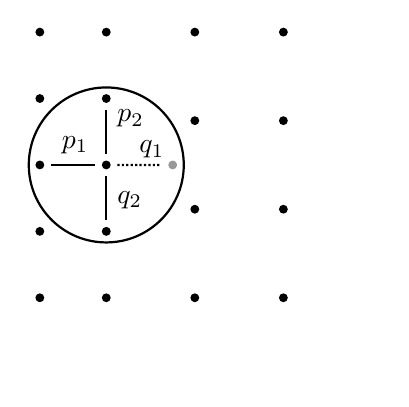
\begin{tikzpicture}[y=0.80pt, x=0.8pt,yscale=-1, inner sep=0pt, outer sep=0pt]
\begin{scope}[shift={(-16.10332,18.79897)}]
  \path[fill=black] (178.797,148.02312) node[above right] (text6246) {};
  \path[shift={(46.10332,-288.79897)},fill=black,nonzero rule] (12.0000,340.0000)
    .. controls (12.0000,341.1046) and (11.1046,342.0000) .. (10.0000,342.0000) ..
    controls (8.8954,342.0000) and (8.0000,341.1046) .. (8.0000,340.0000) ..
    controls (8.0000,338.8954) and (8.8954,338.0000) .. (10.0000,338.0000) ..
    controls (11.1046,338.0000) and (12.0000,338.8954) .. (12.0000,340.0000) --
    cycle;
  \path[shift={(46.10332,-258.79897)},fill=black,fill opacity=0.392,nonzero rule]
    (12.0000,340.0000) .. controls (12.0000,341.1046) and (11.1046,342.0000) ..
    (10.0000,342.0000) .. controls (8.8954,342.0000) and (8.0000,341.1046) ..
    (8.0000,340.0000) .. controls (8.0000,338.8954) and (8.8954,338.0000) ..
    (10.0000,338.0000) .. controls (11.1046,338.0000) and (12.0000,338.8954) ..
    (12.0000,340.0000) -- cycle;
  \path[shift={(46.10332,-318.79897)},fill=black,nonzero rule] (12.0000,340.0000)
    .. controls (12.0000,341.1046) and (11.1046,342.0000) .. (10.0000,342.0000) ..
    controls (8.8954,342.0000) and (8.0000,341.1046) .. (8.0000,340.0000) ..
    controls (8.0000,338.8954) and (8.8954,338.0000) .. (10.0000,338.0000) ..
    controls (11.1046,338.0000) and (12.0000,338.8954) .. (12.0000,340.0000) --
    cycle;
  \path[shift={(46.10332,-348.79897)},fill=black,nonzero rule] (12.0000,340.0000)
    .. controls (12.0000,341.1046) and (11.1046,342.0000) .. (10.0000,342.0000) ..
    controls (8.8954,342.0000) and (8.0000,341.1046) .. (8.0000,340.0000) ..
    controls (8.0000,338.8954) and (8.8954,338.0000) .. (10.0000,338.0000) ..
    controls (11.1046,338.0000) and (12.0000,338.8954) .. (12.0000,340.0000) --
    cycle;
  \path[shift={(46.10332,-258.79897)},fill=black,nonzero rule] (12.0000,340.0000)
    .. controls (12.0000,341.1046) and (11.1046,342.0000) .. (10.0000,342.0000) ..
    controls (8.8954,342.0000) and (8.0000,341.1046) .. (8.0000,340.0000) ..
    controls (8.0000,338.8954) and (8.8954,338.0000) .. (10.0000,338.0000) ..
    controls (11.1046,338.0000) and (12.0000,338.8954) .. (12.0000,340.0000) --
    cycle;
  \path[shift={(46.10332,-228.79897)},fill=black,nonzero rule] (12.0000,340.0000)
    .. controls (12.0000,341.1046) and (11.1046,342.0000) .. (10.0000,342.0000) ..
    controls (8.8954,342.0000) and (8.0000,341.1046) .. (8.0000,340.0000) ..
    controls (8.0000,338.8954) and (8.8954,338.0000) .. (10.0000,338.0000) ..
    controls (11.1046,338.0000) and (12.0000,338.8954) .. (12.0000,340.0000) --
    cycle;
  \path[shift={(16.10332,-288.79897)},fill=black,nonzero rule] (12.0000,340.0000)
    .. controls (12.0000,341.1046) and (11.1046,342.0000) .. (10.0000,342.0000) ..
    controls (8.8954,342.0000) and (8.0000,341.1046) .. (8.0000,340.0000) ..
    controls (8.0000,338.8954) and (8.8954,338.0000) .. (10.0000,338.0000) ..
    controls (11.1046,338.0000) and (12.0000,338.8954) .. (12.0000,340.0000) --
    cycle;
  \path[shift={(16.10332,-318.79897)},fill=black,nonzero rule] (12.0000,340.0000)
    .. controls (12.0000,341.1046) and (11.1046,342.0000) .. (10.0000,342.0000) ..
    controls (8.8954,342.0000) and (8.0000,341.1046) .. (8.0000,340.0000) ..
    controls (8.0000,338.8954) and (8.8954,338.0000) .. (10.0000,338.0000) ..
    controls (11.1046,338.0000) and (12.0000,338.8954) .. (12.0000,340.0000) --
    cycle;
  \path[shift={(16.10332,-348.79897)},fill=black,nonzero rule] (12.0000,340.0000)
    .. controls (12.0000,341.1046) and (11.1046,342.0000) .. (10.0000,342.0000) ..
    controls (8.8954,342.0000) and (8.0000,341.1046) .. (8.0000,340.0000) ..
    controls (8.0000,338.8954) and (8.8954,338.0000) .. (10.0000,338.0000) ..
    controls (11.1046,338.0000) and (12.0000,338.8954) .. (12.0000,340.0000) --
    cycle;
  \path[shift={(16.10332,-258.79897)},fill=black,nonzero rule] (12.0000,340.0000)
    .. controls (12.0000,341.1046) and (11.1046,342.0000) .. (10.0000,342.0000) ..
    controls (8.8954,342.0000) and (8.0000,341.1046) .. (8.0000,340.0000) ..
    controls (8.0000,338.8954) and (8.8954,338.0000) .. (10.0000,338.0000) ..
    controls (11.1046,338.0000) and (12.0000,338.8954) .. (12.0000,340.0000) --
    cycle;
  \path[shift={(16.10332,-228.79897)},fill=black,nonzero rule] (12.0000,340.0000)
    .. controls (12.0000,341.1046) and (11.1046,342.0000) .. (10.0000,342.0000) ..
    controls (8.8954,342.0000) and (8.0000,341.1046) .. (8.0000,340.0000) ..
    controls (8.0000,338.8954) and (8.8954,338.0000) .. (10.0000,338.0000) ..
    controls (11.1046,338.0000) and (12.0000,338.8954) .. (12.0000,340.0000) --
    cycle;
  \path[shift={(86.10332,-348.79897)},fill=black,nonzero rule] (12.0000,340.0000)
    .. controls (12.0000,341.1046) and (11.1046,342.0000) .. (10.0000,342.0000) ..
    controls (8.8954,342.0000) and (8.0000,341.1046) .. (8.0000,340.0000) ..
    controls (8.0000,338.8954) and (8.8954,338.0000) .. (10.0000,338.0000) ..
    controls (11.1046,338.0000) and (12.0000,338.8954) .. (12.0000,340.0000) --
    cycle;
  \path[shift={(86.10332,-308.79897)},fill=black,nonzero rule] (12.0000,340.0000)
    .. controls (12.0000,341.1046) and (11.1046,342.0000) .. (10.0000,342.0000) ..
    controls (8.8954,342.0000) and (8.0000,341.1046) .. (8.0000,340.0000) ..
    controls (8.0000,338.8954) and (8.8954,338.0000) .. (10.0000,338.0000) ..
    controls (11.1046,338.0000) and (12.0000,338.8954) .. (12.0000,340.0000) --
    cycle;
  \path[shift={(86.10332,-268.79897)},fill=black,nonzero rule] (12.0000,340.0000)
    .. controls (12.0000,341.1046) and (11.1046,342.0000) .. (10.0000,342.0000) ..
    controls (8.8954,342.0000) and (8.0000,341.1046) .. (8.0000,340.0000) ..
    controls (8.0000,338.8954) and (8.8954,338.0000) .. (10.0000,338.0000) ..
    controls (11.1046,338.0000) and (12.0000,338.8954) .. (12.0000,340.0000) --
    cycle;
  \path[shift={(86.10332,-228.79897)},fill=black,nonzero rule] (12.0000,340.0000)
    .. controls (12.0000,341.1046) and (11.1046,342.0000) .. (10.0000,342.0000) ..
    controls (8.8954,342.0000) and (8.0000,341.1046) .. (8.0000,340.0000) ..
    controls (8.0000,338.8954) and (8.8954,338.0000) .. (10.0000,338.0000) ..
    controls (11.1046,338.0000) and (12.0000,338.8954) .. (12.0000,340.0000) --
    cycle;
  \path[shift={(126.10332,-348.79897)},fill=black,nonzero rule] (12.0000,340.0000)
    .. controls (12.0000,341.1046) and (11.1046,342.0000) .. (10.0000,342.0000) ..
    controls (8.8954,342.0000) and (8.0000,341.1046) .. (8.0000,340.0000) ..
    controls (8.0000,338.8954) and (8.8954,338.0000) .. (10.0000,338.0000) ..
    controls (11.1046,338.0000) and (12.0000,338.8954) .. (12.0000,340.0000) --
    cycle;
  \path[shift={(126.10332,-308.79897)},fill=black,nonzero rule] (12.0000,340.0000)
    .. controls (12.0000,341.1046) and (11.1046,342.0000) .. (10.0000,342.0000) ..
    controls (8.8954,342.0000) and (8.0000,341.1046) .. (8.0000,340.0000) ..
    controls (8.0000,338.8954) and (8.8954,338.0000) .. (10.0000,338.0000) ..
    controls (11.1046,338.0000) and (12.0000,338.8954) .. (12.0000,340.0000) --
    cycle;
  \path[shift={(126.10332,-268.79897)},fill=black,nonzero rule] (12.0000,340.0000)
    .. controls (12.0000,341.1046) and (11.1046,342.0000) .. (10.0000,342.0000) ..
    controls (8.8954,342.0000) and (8.0000,341.1046) .. (8.0000,340.0000) ..
    controls (8.0000,338.8954) and (8.8954,338.0000) .. (10.0000,338.0000) ..
    controls (11.1046,338.0000) and (12.0000,338.8954) .. (12.0000,340.0000) --
    cycle;
  \path[shift={(126.10332,-228.79897)},fill=black,nonzero rule] (12.0000,340.0000)
    .. controls (12.0000,341.1046) and (11.1046,342.0000) .. (10.0000,342.0000) ..
    controls (8.8954,342.0000) and (8.0000,341.1046) .. (8.0000,340.0000) ..
    controls (8.0000,338.8954) and (8.8954,338.0000) .. (10.0000,338.0000) ..
    controls (11.1046,338.0000) and (12.0000,338.8954) .. (12.0000,340.0000) --
    cycle;
  \path[fill=black] (36.103317,46.201031) node[above right] (text4184) {$p_1$};
  \path[fill=black] (71.103317,48.201031) node[above right] (text4188) {$q_1$};
    \path[color=black,fill=black,line width=0.800pt] (31.1033,50.7010) --
      (31.1033,51.7010) -- (51.1033,51.7010) -- (51.1033,50.7010) --
      (31.1033,50.7010) -- cycle;
    \path[line join=round,even odd rule,line width=0.500pt] (33.0289,52.4112) --
      (29.7511,51.2058) -- (33.0289,50.0005) .. controls (32.5052,50.7121) and
      (32.5083,51.6858) .. (33.0289,52.4112) -- cycle;
    \path[color=black,fill=black,line width=0.800pt] (55.6033,56.2010) --
      (55.6033,76.2010) -- (56.6033,76.2010) -- (56.6033,56.2010) --
      (55.6033,56.2010) -- cycle;
    \path[line join=round,even odd rule,line width=0.500pt] (57.3134,74.2755) --
      (56.1081,77.5532) -- (54.9028,74.2755) .. controls (55.6144,74.7991) and
      (56.5880,74.7961) .. (57.3134,74.2755) -- cycle;
    \path[color=black,fill=black,line width=0.800pt] (55.6033,26.2010) --
      (55.6033,46.2010) -- (56.6033,46.2010) -- (56.6033,26.2010) --
      (55.6033,26.2010) -- cycle;
    \path[line join=round,even odd rule,line width=0.500pt] (54.8932,28.1266) --
      (56.0985,24.8488) -- (57.3038,28.1266) .. controls (56.5922,27.6030) and
      (55.6186,27.6060) .. (54.8932,28.1266) -- cycle;
    \path[color=black,fill=black,line width=0.800pt] (61.1033,51.7010) --
      (62.1033,51.7010) -- (62.1033,50.7010) -- (61.1033,50.7010) --
      cycle(63.1033,51.7010) -- (64.1033,51.7010) -- (64.1033,50.7010) --
      (63.1033,50.7010) -- cycle(65.1033,51.7010) -- (66.1033,51.7010) --
      (66.1033,50.7010) -- (65.1033,50.7010) -- cycle(67.1033,51.7010) --
      (68.1033,51.7010) -- (68.1033,50.7010) -- (67.1033,50.7010) --
      cycle(69.1033,51.7010) -- (70.1033,51.7010) -- (70.1033,50.7010) --
      (69.1033,50.7010) -- cycle(71.1033,51.7010) -- (72.1033,51.7010) --
      (72.1033,50.7010) -- (71.1033,50.7010) -- cycle(73.1033,51.7010) --
      (74.1033,51.7010) -- (74.1033,50.7010) -- (73.1033,50.7010) --
      cycle(75.1033,51.7010) -- (76.1033,51.7010) -- (76.1033,50.7010) --
      (75.1033,50.7010) -- cycle(77.1033,51.7010) -- (78.1033,51.7010) --
      (78.1033,50.7010) -- (77.1033,50.7010) -- cycle(79.1033,51.7010) --
      (80.1033,51.7010) -- (80.1033,50.7010) -- (79.1033,50.7010) -- cycle;
    \path[line join=round,even odd rule,line width=0.500pt] (79.1777,49.9909) --
      (82.4555,51.1962) -- (79.1777,52.4015) .. controls (79.7014,51.6899) and
      (79.6984,50.7163) .. (79.1777,49.9909) -- cycle;
  \path[shift={(76.10332,-288.79897)},fill=black,fill opacity=0.404,nonzero rule]
    (12.0000,340.0000) .. controls (12.0000,341.1046) and (11.1046,342.0000) ..
    (10.0000,342.0000) .. controls (8.8954,342.0000) and (8.0000,341.1046) ..
    (8.0000,340.0000) .. controls (8.0000,338.8954) and (8.8954,338.0000) ..
    (10.0000,338.0000) .. controls (11.1046,338.0000) and (12.0000,338.8954) ..
    (12.0000,340.0000) -- cycle;
  \path[shift={(16.10332,-38.79897)},draw=black,fill=black,line join=round,miter
    limit=4.00,fill opacity=0.000,nonzero rule,line width=0.800pt]
    (75.0000,90.0000) .. controls (75.0000,109.3300) and (59.3300,125.0000) ..
    (40.0000,125.0000) .. controls (20.6700,125.0000) and (5.0000,109.3300) ..
    (5.0000,90.0000) .. controls (5.0000,70.6700) and (20.6700,55.0000) ..
    (40.0000,55.0000) .. controls (59.3300,55.0000) and (75.0000,70.6700) ..
    (75.0000,90.0000) -- cycle;
  \path[fill=black] (61.103317,34.201031) node[above right] (text5037) {$p_2$};
  \path[fill=black] (61.103317,71.201027) node[above right] (text5041) {$q_2$};
\end{scope}

\end{tikzpicture}


  \caption{Virtual Points Pair Up Unpaired Neighbors}
  \label{fig:virtualpoint}
\end{figure}
%
Note that, while bonds \(p_2\) and \(q_2\) form a perfect bond pair, there is no bond exactly opposite \(p_1\).
To solve this, we add a virtual point to create a bond, \(q_1\), that will form a pair with \(p_1\).
Because this point is not part of the discretization, it has no mass, and its properties must be determined from the properties of the surrounding nodes.
An easy method of determining properties (such as displacement) at virtual nodes is to use a weighted average.
One method of generating useful weights that is relatively robust is barycentric interpolation.
We start by finding the three (non-colinear) real nodes closest to the location of the virtual node, A, B, and C.
Next, we find the signed areas of the triangles ABC, ABX, BCX, and CAX, with X being the virtual node.
The weight of node A is the area ratio between BCX and ABC, the weight of node B is the ratio of areas CAX and ABC, and the weight of node C is the ratio of areas ABX to ABC.
Using signed areas allows the weights to be negative to extrapolate properties of a virtual node outside of ABC.
Because these weights are calculated from the initial positions of the node, they can be stored for swift evaluation of properties at virtual nodes.

%
\begin{figure}[tbp]
  \centering
  


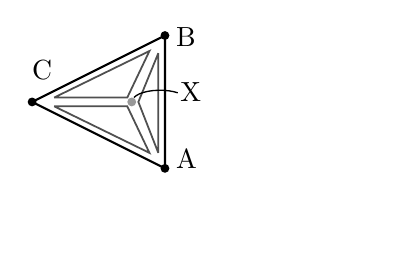
\begin{tikzpicture}[y=0.80pt, x=0.8pt,yscale=-1, inner sep=0pt, outer sep=0pt]
\begin{scope}[shift={(-16.10332,-41.20103)}]
  \path[fill=black] (178.797,148.02312) node[above right] (text6246) {};
  \path[shift={(16.10332,-258.79897)},fill=black,nonzero rule] (12.0000,340.0000)
    .. controls (12.0000,341.1046) and (11.1046,342.0000) .. (10.0000,342.0000) ..
    controls (8.8954,342.0000) and (8.0000,341.1046) .. (8.0000,340.0000) ..
    controls (8.0000,338.8954) and (8.8954,338.0000) .. (10.0000,338.0000) ..
    controls (11.1046,338.0000) and (12.0000,338.8954) .. (12.0000,340.0000) --
    cycle;
  \path[shift={(76.10332,-288.79897)},fill=black,nonzero rule] (12.0000,340.0000)
    .. controls (12.0000,341.1046) and (11.1046,342.0000) .. (10.0000,342.0000) ..
    controls (8.8954,342.0000) and (8.0000,341.1046) .. (8.0000,340.0000) ..
    controls (8.0000,338.8954) and (8.8954,338.0000) .. (10.0000,338.0000) ..
    controls (11.1046,338.0000) and (12.0000,338.8954) .. (12.0000,340.0000) --
    cycle;
  \path[shift={(76.10332,-228.79897)},fill=black,nonzero rule] (12.0000,340.0000)
    .. controls (12.0000,341.1046) and (11.1046,342.0000) .. (10.0000,342.0000) ..
    controls (8.8954,342.0000) and (8.0000,341.1046) .. (8.0000,340.0000) ..
    controls (8.0000,338.8954) and (8.8954,338.0000) .. (10.0000,338.0000) ..
    controls (11.1046,338.0000) and (12.0000,338.8954) .. (12.0000,340.0000) --
    cycle;
  \path[shift={(61.10332,-258.79897)},fill=black,fill opacity=0.404,nonzero rule]
    (12.0000,340.0000) .. controls (12.0000,341.1046) and (11.1046,342.0000) ..
    (10.0000,342.0000) .. controls (8.8954,342.0000) and (8.0000,341.1046) ..
    (8.0000,340.0000) .. controls (8.0000,338.8954) and (8.8954,338.0000) ..
    (10.0000,338.0000) .. controls (11.1046,338.0000) and (12.0000,338.8954) ..
    (12.0000,340.0000) -- cycle;
  \path[fill=black] (91.103317,111.20103) node[above right] (text3133) {A};
  \path[fill=black] (91.103317,56.201031) node[above right] (text3137) {B};
  \path[fill=black] (26.103317,71.201027) node[above right] (text3141) {C};
  \path[shift={(16.10332,-18.79897)},draw=black,line join=miter,line cap=butt,line
    width=0.800pt] (10.0000,100.0000) -- (70.0000,70.0000) -- (70.0000,130.0000)
    -- cycle;
  \path[shift={(16.10332,-18.79897)},draw=black,line join=miter,line
    cap=butt,miter limit=4.00,draw opacity=0.686,line width=0.640pt]
    (20.0000,98.0000) -- (63.0000,77.0000) -- (53.0000,98.0000) -- cycle;
  \path[shift={(16.10332,-18.79897)},draw=black,line join=miter,line
    cap=butt,miter limit=4.00,draw opacity=0.686,line width=0.640pt]
    (67.0000,78.0000) -- (58.0000,100.0000) -- (67.0000,123.0000) -- cycle;
  \path[shift={(16.10332,-18.79897)},draw=black,line join=miter,line
    cap=butt,miter limit=4.00,draw opacity=0.686,line width=0.640pt]
    (20.0000,102.0000) -- (53.0000,102.0000) -- (63.0000,123.0000) -- cycle;
  \path[fill=black] (93.103317,81.201027) node[above right] (text3157) {X};
  \path[shift={(-8.65052,-9.08887)},draw=black,fill=black,line join=round,miter
    limit=4.00,fill opacity=0.000,nonzero rule,line width=0.480pt]
    (80.7538,88.2899) .. controls (83.1150,85.6950) and (90.2880,84.3571) ..
    (96.7753,85.3015) .. controls (98.1455,85.5010) and (99.4178,85.7949) ..
    (100.5349,86.1698);
\end{scope}

\end{tikzpicture}


  \caption{Barycentric interpolation is based on the relative areas of sub triangles}
  \label{fig:BaryCentric}
\end{figure}
%

With the properties of the virtual points determined, the model can be evaluated in the same manner as the uniformly discretized models of the previous papers.
Where forces are calculated to act on a virtual node, those forces are redistributed to the supporting real nodes according to the weight each point has in the interpolation.

The same method of virtual nodes also allows the modeling of curved surfaces, in which the perfect opposite of a bond may not lie near but not on the surface of the plate or shell.
As long as the curvature of the surface is small (at the scale of the peridynamic horizon), each resulting virtual nodes will be nearly in the plane formed by its nearest neighbors.
Finding the weights of the surrounding nodes is performed just as in the planar case, except that the areas are formed between the projection of the virtual node location X onto the plane formed by A, B, and C.

%%
%\begin{figure}[tbp]
%  \centering
%  \input{\diagrampath/VirtualCurve.tex}
%  \caption{Virtual Points Allow Straight Pairs on Curved Surfaces}
%  \label{fig:virtualcurve}
%\end{figure}
%%

To compute the weight of node A in the interpolation of properties at virtual node X, let AB represent the vector from node A to node B, and use
%
\begin{equation}
\label{eq:BarycentricArea}
W'_A = \frac{B-X}{2}\bullet \left[BC \times \left(\frac{BC \times BA}{|BC \times BA|}\right)\right]
\end{equation}
%
After finding $W'_B$ and $W'_C$ in similar fashion,
%
\begin{equation}
\label{eq:BarycentricWeight}
W_A = \frac{W'_A }{W'_A + W'_B + W'_C}
\end{equation}
%
If the projection of X onto the plane defined by A, B, and C lies outside the triangle ABC,  one or two of $W_A$, $W_B$ and $W_C$ will be negative, though they will still sum to 1.

\section{``Boundary'' Conditions}
Because peridynamic models result in long range forces, it is not sufficient to apply boundary conditions to nodes on the relevant boundary; nodes near the boundary must be considered as well.
Displacement conditions are enforced on the nodes nearest to a simply-supported plate edge, while average displacements are enforced on a small collection of nodes surrounding a beam pin support.
Clamped boundary conditions are simulated by controlling the displacement of 1-5 nodes nearest the boundary and applying a symmetry boundary condition to nodes out to a distance of \(2\delta\) from the boundary. 
Point loads are evenly distributed over all nodes in a region with width or diameter of \(\delta\) centered on the point load location.
Line and pressure loads are treated normally.

\section{Numerical Solution Method}

This project uses Trilinos, a collection of open software libraries, or packages, from Sandia National Labs, including:
\begin{itemize}
  \item Epetra and EpetraExt - provide efficient parallel data structures, particularly vectors and sparse matrices
  \item Isorropia - provides load balancing, partitioning, and matrix coloring
  \item NOX - a collection of large-scale nonlinear system solver utilities
  \item PyTrilinos - a python interface providing Python wrappers for many Trilinos packages, and offering compatibility between numpy.ndarrays and Epetra.MultiVectors
\end{itemize}

The nature of discrete peridynamic models results in large numbers of parallelizable computations.
Efficient parallelization is achieved using Epetra data structures for distributed variables.
Model force evaluations are coded in Python, making extensive use of the optimized routines in the NumPy and SciPy packages operating on the distributed Epetra objects. 
To obtain quasistatic solutions, problems are coded into NOX objects and solved using NOX nonlinear solvers.
Preliminary analysis was performed using a Newton Method solver on an iMac with a 3.1GHz Intel Core i7 processor and 16GB RAM, using 1-4 cores.
The nature of the Trilinos packages and the structure of the code allow for more extensive parallel computation without major code changes.

For all but the simplest loading conditions, analytical solutions to boundary condition problems become complicated.
As load conditions and material behavior become more complex, there are no analytical solutions.
For comparison, equivalent models are created and analyzed in Abaqus 6.12 to verify simple cases.
